Nach der Problemanalyse und der Untersuchung auf Ansatzpunkte für eine mögliche Optimierung des Prozesses, folgt in diesem Kapitel nun die Überführung dieser Gedanken in Konzepte zur praktischen Umsetzung. Dabei wird untersucht, welche theoretischen Verfahren geeignet wären, um die herausgearbeiteten Anforderungen zu erfüllen. Außerdem wird für potentiell passende Verfahren auch schon eine technische Lösung zur prototypische Implementierung geplant.

\subsection{Anforderungsanalyse}
\todo{Weitere Anforderungen?}

In diesem Kapitel werden zunächst einmal die Kernanforderungen und die Ziele dieser Entwicklungsarbeit zusammengetragen.

Die Hauptaufgabe, weshalb der ganze Aufwand überhaupt betrieben werden soll, ist die verbesserte Einplanung von ankommenden LKW am Terminal. Ziel ist es, durch gezielte Planung der Ankunftszeiten, eine schnellere bzw. effizientere Abfertigung zu realisieren und dadurch insgesamt Zeiteinsparungen zu erreichen, welche dann genutzt werden können, um zusätzliche LKW zu bearbeiten. Dieses Ziel soll mit Hilfe einer softwarebasierten Lösung erreicht werden, es sollen also passende Algorithmen geplant und entwickelt werden. In vorherigen Kapiteln wurden bereits die wesentlichen und am meisten Gewinn versprechenden Optimierungspotentiale herausgearbeitet. Erste umfangreichere Recherchen haben allerdings gezeigt, dass es sehr schwierig sein wird, eine Lösung zu finden, welche all diese Punkte berücksichtigt. Ein eigenes und speziell angepasstes Verfahren zu entwickeln, ist kaum machbar, sodass es das Ziel sein muss, bewährte Verfahren zu finden, welche auf das vorliegende Problem adaptiert werden können. So ist es möglich bereits bekannte Lösungswege zu nutzen. Aus diesem Grund wird im folgenden eher abzuwägen sein, welche dieser Ansätze überhaupt auf die Anforderungen passen, ob sich möglicherweise kombinieren lassen und wie sich diese dann in einer Software umsetzen lassen.

Um den Umfang dieser prototypischen Entwicklung überschaubar zu halten und den Fokus auf den Kern, der Entwicklung von Optimierungen zu lenken, sollen hier auch wirklich nur dafür Konzepte erarbeitet und umgesetzt werden. Rahmenfunktinalitäten, wie die Eingabe von Avisierungen oder auch die Kommunikation der geplanten Zeiten mit den Speditionen und LKW Fahrern, welche in einer real einsetzbaren Software möglicherweise benötigt werden, sollen an dieser Stelle nicht betrachtet werden.

Wichtigster Aspekt, um eine sinnvolle Planung durchführen zu können ist es, eine gute Datenbasis zu schaffen. Dem Planungsalgorithmus muss also eine Liste von Datensätzen übergeben werden, die jeweils alle Buchungen für einen Zeitslot enthalten. Welche Details das genau sind, wird auch von dem nachfolgend geplanten Algorithmus abhängen. Um aber einen guten und sinnvollen Eindruck des ankommenden Gutes zu erhalten, wird ein solcher Eingabedatensatz aber sicherlich folgende Informationen enthalten müssen:
\begin{itemize}
    \item Liefergutart
    \item Warenbeschreibung
    \item Buchungsnummer
    \item Ausmaße der Ware: Länge, Breite, Höhe, Gewicht
    \item Kategorie der Be- oder Entladung (zur Bestimmung der benötigten Ladehilfsmittel und Ressourcen)
\end{itemize}
Ein Optimierungsalgorithmus muss aus diesen Daten für jeden LKW eine genaue Ankunftszeit festlegen und ausgeben. Die genaue Art und Weise der Planung wird noch zu untersuchen sein, es wird allerdings kaum umgänglich sein, zunächst alle Buchungen mit einer groben Vorstellung des Zeitfensters zu sammeln und im Nachgang eine genaue Zeit festzulegen. Andernfalls wird es wieder viel Spielraum und Zufallsvariablen geben, die eine Optimierung des aktuellen Zustands nahezu unmöglich machen. Bezüglich der Datenbasis und der Art der ankommenden LKW wird für diese Arbeit festgelegt, dass jeder LKW nur eine Art bzw. Kategorie von Ladegut enthalten kann. Wie aus Experteninterviews (siehe Anhang \ref{sec:appendixInterviews} \todo{richtige ref}) hervor ging, können LKW theoretisch mehrere unterschiedliche Güter enthalten und somit zu mehreren bzw. entsprechend besonders ausgewählten und passenden Ladeplätzen fahren müssen. Dies erscheint eine sehr spezielle Randbedingung zu sein, welche einer strukturierten Eingabe und Verarbeitung sehr im Weg steht und deshalb hier zunächst einmal nicht weiter berücksichtigt werden soll.

Eine weitere einschränkende Anforderung bzw. Festlegung für den hier entwickelten Algorithmus ist es, dass die Art der Buchungen auf anliefernde LKW beschränkt wird. Auch hier ist die Idee, die Entwicklung strukturierter und übersichtlicher zu halten, dass zwangsweise jede kleinste Anforderung zu berücksichtigen ohne dass anschließend keine gute bzw. eher chaotische Lösung entsteht. Der Fall der Beladung von LKW bringt nur noch weitere zu berücksichtigende Aspekte hinein. Z.B. ist hier die Art des Gutes bekannt, aber nicht unbedingt der LKW, welche beladen werden muss. Es erscheint also sinnvoll, sich zunächst auf den einen Teil der Entladung zu konzentrieren. Die grundsätzlichen Planungsverfahren werden sicherlich in beiden Fällen anwendbar sein und könnten zu einem späteren Zeitpunkt immernoch entsprechend adaptiert werden.

Ein letzter Aspekt, welcher konkret bezogen auf einen möglichen Algorithmus berücksichtigt werden sollte, ist das Zeitverhalten bei der Ausführung. Grundsätzlich ist es so, dass eine schnelle Berechnung besser dafür geeignet ist, eine Berechnung in Echtzeit, bzw. zumindest nahezu Echtzeit zu berechnen. Dies könnte z.B. nützlich sein, um direkt bei der Buchung von Slots sagen zu können, ob ein LKW noch in den LKW passt, und so direkt zu zeigen welche Slots real verfügbar sind. Ergeben sich z.B. kurzfristige Veschiebungen im Zeitplan, so wäre zumindest theoretisch denkbar mit einem schnellen Algorithmus in kurzer Zeit eine Ersatzplanung zu erzeugen. Fraglich wäre allerdings ohnehin, ob es so kurzfristig möglich ist, Ankunftszeiten späterer LKWs vorzuverlegen oder ganz neue LKWs einzuplanen. Vermutlich wird das für mehr Durcheinander sorgen, als dass es am Ende Vorteile bringt. Aus diesem Grund ist eine schnelle Verarbeitungszeit zu bevorzugen, allerdings wird ein langsamer Algorithmus, welcher möglicherweise über Nacht oder einige Tage im Voraus arbeiten kann, um einen besseren Plan zu erzeugen auch akzeptabel sein. Es ist ohnehin zu bedenken, dass eine möglichst genaue und auch zuverlässige Anmeldung und Ankunft der LKW für den ganzen Optimierungsprozess wichtig ist. Wenn es also sehr regelmäßig zu kurzfristigen Änderungen kommt, wäre ohnehin abzuwägen, wie praxistauglich die gefundene Lösung ist. Ohne zuverlässiges Vorwissen ist es einfach sehr schwer Verbesserungen zu erzielen.


\subsection{Vergleich von Lösungsansätzen}

Die Idee zum weiteren Vorgehen ist es nun, einen Algorithmus zu planen, welcher die zuvor herausgearbeiteten Anforderungen und Ziele erfüllen kann. Es soll also möglich sein, einen vorgegebenen Satz von Buchungen in einen derartigen Zeitplan zu überführen, dass möglichst wenig Zeit benötigt wird, bzw. dass möglichst viele zusätzliche LKW abgearbeitet werden können als es bisher der Fall ist. Die Schwierigkeit, die sich dabei vor allem ergibt ist, dass es extrem schwer ist, alle zuvor genannten Rahmenbedingungen, Regeln und Einflussfaktoren in einem einzigen Algorithmus zu vereinen. Aus diesem Grund ist der Ansatz zum Finden einer geeigneten Lösung, bekannte Probleme zu recherchieren und zu nutzen bzw. diese zumindest soweit abzuwandeln, dass sich bekannte und bereits gut erforschte Lösungen anwenden lassen. Dies verringert den Arbeitsaufwand enorm und führt gleichzeitig zu einer wesentlich höheren Erfolgsaussicht. Derartige Verfahren wurden bereits vielfach getestet. Außerdem wäre es kaum machbar oder auf alle Fälle extrem aufwändig und in dieser Arbeit vermutlich kaum schaffbar, umfangreiche Eigenentwicklungen anzustellen.

Die zum Finden einer Lösung angestellten Recherchen haben verschiedene, mehr oder minder gute Ansatzpunkte ergeben. Die werden nachfolgend zusammengetragen und bei Erfolgsaussichten auch weiter ausgearbeitet. Ein erster allgemeiner Startpunkt war die Idee zur Nutzung von künstlicher Intelligenz. Dies stellte sich allerdings bei näheren Gedanken zur Umsetzung als eher schwierig heraus, sodass zwei Ideen weitere erarbeitet wurden, wie ein entsprechender Algorithmus aussehen könnte. Beide berücksichtigen unterschiedliche Aspekte aus der Analyse der Optimierungspotenziale (siehe Kapitel \ref{sec:analyseOptimierungspotenziale}). Da es schwierig ist, einen Algorithmus zu planen, welcher alle Aspekte berücksichtigt, wurden im Folgenden beide Ansätze ausführlich recherchiert und geplant. Es soll eine parallele Implementierung und ein direkter Vergleich folgen, um so möglichst viele Ideen zur Optimierung abzudecken und hinterher eine Bewertung der vielversprechendsten Methoden zu erzielen.

\subsubsection{Lösung mittels künstlicher Intelligenz}

Wie bereits herausgearbeitet wurde, handelt es sich bei der vorliegenden Aufgabe um ein sehr komplexes Problem mit vielen Einflussfaktoren. Ein in den letzten Jahren sehr populär gewordener und weit verbreiteter Ansatz, um solche Probleme zu lösen, ist die künstliche Intelligenz (KI). Deshalb ist dies auch hier ein Ansatz, der nachfolgend genauer beleuchtet werden soll. Prinzipiell ist die Idee künstlicher Intelligenz, Computer Dinge machen zu lassen, bei denen Menschen bisher besser waren. Maschinen sollen also die Fähigkeit bekommen, kognitive Aufgaben zu erfüllen, bei denen es bisher immer noch nötig war, den menschlichen Verstand zu nutzen. Dabei gibt es Aufgaben die für Menschen deutlich schwerer sind als für Computer, so z.B. mathematische Zusammenhänge verstehen und berechnen. Erkennung von Sprache oder Bildern fällt Menschen dagegen sehr leicht, während es eine große Herausforderung für Computer darstellt, einen tieferen Sinn zu erkennen. Zur technischen Umsetzung braucht ein Computer irgendeine Form von Modell, um ein \glqq{}intelligentes\grqq{} Verhalten durch Berchnungen auf einem Prozessor nachbilden zu können. Ein Beispiel dafür sind \textit{neuronale Netze}. Sie versuchen das menschliche Nervensystem zu adaptieren und durch verschiedene, nicht-lineare Funktionen nachzubilden. Um solche Modelle dazu zu bringen, \glqq{}intelligent\grqq{} zu sein und in den für sie vorgesehenen Situationen die richtigen Entscheidungen zu treffen, braucht es ein sogenanntes Training. Lernt man das System zunächst mit einer Vielzahl von Daten aus Erfahrungswerten an, kann es dadurch lernen Muster zu erkennen und diese auf unbekannte Eingabedaten anzuwenden. \cite{KIverstehen}

Die grundlegende Idee für dieses Beispiel ist es, die KI so trainieren, dass sie alle nötigen Zusammenhänge des Problems selbstständig erkennen und auf zukünftige Eingaben anwenden kann. So müssten nicht alle Details und Randbedingungen manuell erfasst und implementiert werden. Die Voraussetzung dafür ist, dass es bereits eine große Datenbasis zum Training gibt. Hier ergibt sich allerdings auch schon das große Problem in diesem Fall: Die verfügbare Datengrundlage ist im vorliegenden Beispiel leider nicht gegeben. Zum einen gibt so gut wie keine realen Daten, auf die zurückgegriffen werden kann. Wie schon erkannt wurde, sind die aktuell erfassten Daten aber auch gar nicht geeignet, um zuverlässig eine gute Bestimmung der benötigten Zeit und Ressourcen zu erzeugen. Und da eine KI auch nicht zaubern kann, wird auch sie daraus keine zuverlässig Guten Ergebnisse erzielen können. D.h. es wäre höchstens möglich, eine Reihe von fiktiven Datensätzen zu erzeugen, wie sie potenziell in der Realität vorkommen. Das wäre zum einen ein extremer Zeitaufwand, da zum zuverlässigen Training einer KI eine extrem hohe Zahl von Beispieldatensätzen benötigt wird. Zusätzlich ist dann fraglich, ob diese fiktiven Daten ein reales Problem zuverlässig und in all seinen Dimensionen abbilden können. Hinzu kommt, dass auch in irgendeiner Form erfasst und der KI mitgeteilt werden müsste, wie das gewünschte, beste Ergebnis zu den jeweiligen Eingabedaten ist. Einfach einen Satz von eingegebenen Buchungen zu übergeben und der KI zu sagen: \glqq{}Finde das beste Ergebnis\grqq{}, funktioniert nicht. Es sind also sehr aufwändige Schritte und Gedanken notwendig, beispielsweise: Welche Art von KI und welches Modell soll überhaupt genutzt werden? Wie kann solche man eine entsprechende praktisch Implementierung umsetzen? Wie sollen die Ergebnisse bzw. Ausgaben aussehen? Wie und mit welchen Daten läuft ein Training ab? Und viele mehr. \cite{KIverstehen}

Insgesamt würde zur weiteren Verfolgung dieses Ansatzes sehr viel Zeit in die Einarbeitung, Entwicklung und das Training einer KI fließen. Bei bisher eher begrenzter Erfahrung in diesem Bereich und einer so ungewissen Ausgangssituation, ist ein Erfolg in gegebener Zeit eher fraglich. Aus diesem Grund wurde dieser Ansatz auch nicht umfangreicher verfolgt und mit dieser kurzen Recherche abgeschlossen.

\subsubsection{Algorithmus 1: Planung der Ressourcen}

Aus zuvor genannten Gründen wurde sich daher auf spezifischere Ideen zur Umsetzung konzentriert. Der Ansatz dieser Variante ist es, alle auf dem Terminalgelände zur Verfügung stehenden Ressourcen zu erfassen und in einem Zeitplan möglichst optimal auf die angemeldeten LKW zu verteilen. Grundvoraussetzung ist hier auf jeden Fall eine gute und vollständige Anmeldung, sodass bereits bei der Planung klar ist, welche Ressourcen durch welchen Auftrag gebunden werden. Der Gedanke ist hier, dass durch eine freie Planung innerhalb des vorausgewählten Slots eine deutlich effektivere und höhere Ausnutzung der Ressourcen erzielt werden kann, als wenn die LKW einfach zufällig kommen. Wenn Ressourcen nicht für einen Großteil des Slots benötigt werden, könnte deren Nutzungszeit zumindest auf einen möglichst engen Zeitraum begrenzt werden, um die Leerlaufzeit zu minimieren und sie möglicherweise für ganz andere Arbeiten verfügbar zu machen. Es müssen aber noch einige weitere Rahmenbedingungen und Annahmen für diesen Ansatz gesetzt werden. So ist es für eine gute Planung wichtig, eine möglichst genaue Einschätzung darüber zu haben, welche Ressourcen jeweils benötigt werden und wie lange die Bearbeitung welches LKWs dauert, d.h. wie lange jede Ressource pro Auftrag gebunden ist. Idee wäre es hier, alle Ressourcen auf einer Art Zeitachse einzuplanen. Dabei ist die Besonderheit, dass ein Job mehrere Ressourcen parallel benötigt (vgl. Abb. \ref{fig:rsExampleSchedule}). Eine direkte Unterscheidung und Zuordnung der Ressourcen zu Ladeplätzen, wie es sie bisher im Hafen gibt, wird es für diese Betrachtung zunächst nicht geben. Es wird also mit einer festen Menge von Ressourcen für den gesamten Hafen geben, welche flexibel zu ihrem benötigten LKW zugeordnet werden.
\begin{figure}[H]
    \centering
    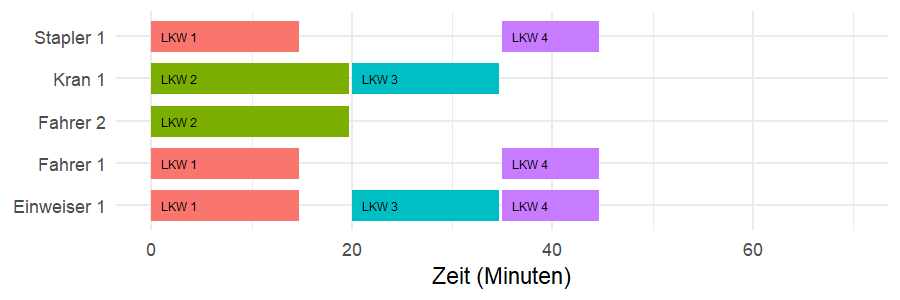
\includegraphics[width=\textwidth]{images/timelines/rsExampleSchedule.png}
    \caption{Beispielhafter Zeitplan für die Ressourcennutzung der Buchungen}
    \label{fig:rsExampleSchedule}
\end{figure}

Der Ansatz zur Umsetzung bzw. zur Lösung des beschriebenen Problems wäre es nun also, einen passenden Scheduling Algorithmus zu finden und möglicherweise leicht anzupassen. Dies stellte sich allerdings bei genauerer Recherche als gar nicht so einfach heraus, wie es im ersten Moment klingt. Es handelt sich hier schon um einen sehr speziellen Anwendungsfall mit einigen besonderen Anforderungen. Im ersten Moment könnte man beim Stichwort Scheduling Algorithmus an diverse Verfahren denken, wie sie z.B. in der Aufgabenverteilung bei Prozessoren vorkommen. Im Unterschied zu den meisten dafür gefundenen Verfahren, werden hier mehrere Ressourcen immer parallel belegt und nicht nacheinander. Dadurch lassen sich die meisten Verfahren hier nicht anwenden. Im folgenden werden einige genauer betrachtete und in diesem Zusammenhang bedeutende Möglichkeiten näher betrachtet und bewertet. Viele hatten allerdings gemeinsam, dass sie nur mit extremer Abwandlung des Algorithmus oder des Problems anwendbar wären. Dann hätte die darauf aufbauende Lösung allerdings kaum noch etwas mit dem eigentlichen Problem und Ziel dieser Arbeit zu tun.

\textbf{Job Shop Scheduling}
\todo{NP-schwer erwähnen?!}

Ein verbreitetes Optimierungsproblem, welches durchaus auch gewisse Ähnlichkeit zu dem hier dargestellten Problem hat, ist das Job-Shop Scheduling, auch als Job-Shop Problem (JSP) bekannt. Ziel dieses Verfahrens ist es, eine Maschinenbelegung zu planen. Ein Beispiel für einen so optimierten Produktionsprozess ist in Abb. \ref{fig:job_shop_skizze} dargestellt. Jeder Job muss dabei nacheinander mehrere Maschinen belegen. Im Beispiel muss jedes Blatt Papier durch alle Druckmaschinen mit den Farben Grün, Blau und Gelb laufen. Dafür soll eine optimale Reihenfolge gefunden werden, wann welcher Job auf welcher Maschine bearbeitet wird, sodass die gesamte Produktionsdauer möglichst gering ist. Der Prozess kann aber auch komplexer sein. Verschiedene Jobs können auch unterschiedliche Maschinen benötigen. Es sind in Varianten des JSP u.a. auch doppelte Maschinen oder eine feste Reihenfolge der Abarbeitung möglich. \cite{jobshop1}

\begin{figure}[H]
    \centering
    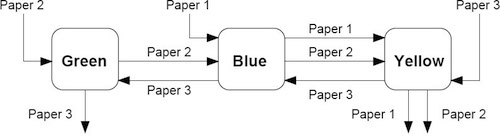
\includegraphics[width=0.8\textwidth]{images/jobshopdiagram.jpg}
    \caption{Beispielhafte Produktion zur Planung mit Job Shop Scheduling \cite{jobshop2}}
    \label{fig:job_shop_skizze}
\end{figure}

Ein daraus resultierender Zeitplan ist beispielhaft in Abbildung \ref{fig:job_shop_schedule} dargestellt. Für jede Maschine wurden hier ein Zeitfenster bestimmt, wann sie für welchen Job arbeitet. Dadurch, dass die Bearbeitungszeiten sehr große Unterschiede haben können, ist eine gute Verteilung wichtig, damit sich möglichst wenige Jobs gegenseitig blockieren und die Gesamtzeit des Plans verkürzt werden kann.

\begin{figure}[H]
    \centering
    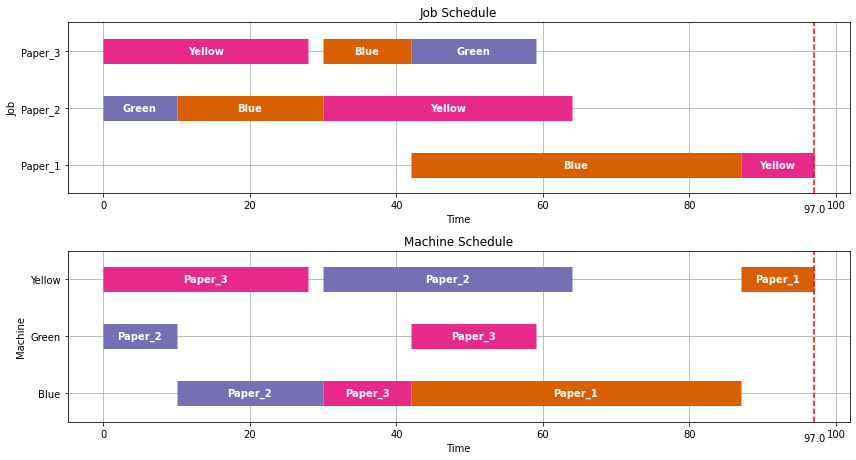
\includegraphics[width=\textwidth]{images/jobshopdiagram_schedule.png}
    \caption{Mittels Job-Shop-Verfahren ermittelter Zeitplan der Produktion \cite{jobshop2}}
    \label{fig:job_shop_schedule}
\end{figure}

Der große Vorteil bei der Nutzung des JSP wäre, dass zum einen die Modellierung sehr standardisiert und somit einfach machbar ist. Zum anderen gibt es auch bereits diverse Libraries für die gängigsten Programmiersprachen (bspw. für Python siehe \cite{jobshop2}). Dies macht auch die Umsetzung sehr einfach, da weniger Eigenarbeit nötig ist und auch alle Funktionen bereits vielfach getestet worden sein dürften.

Prinzipiell ist dieser Ansatz deswegen ein sehr vielversprechendes Verfahren. Würde man die im Terminal verfügbaren Ressourcen und Ladehilfsmittel als Maschinen im Sinne des Job-Shop Problems sehen und jeden LKW als Job, welcher durch bestimmt Ressourcen abgearbeitet werden muss, so klingt dies durchaus passend. Auch die Art und Weise des resultierenden Zeitplans ist sicherlich eine sehr gute Darstellung, wie die Belegungszeiten verschiedener Ressourcen eingeteilt werden können. Das große Problem ist allerdings, dass das Job-Shop Verfahren davon ausgeht, dass die Bearbeitung durch die Maschinen nacheinander erfolgt. In dem in dieser Arbeit vorliegenden Problem, müssen die Ressourcen aber immer zeitgleich belegt werden. Es wird beispielsweise immer ein Gabelstapler mit Einweiser zusammen benötigt. Es macht hier keinen Sinn eine Palette zunächst abzuladen und später erst einen Einweiser zu holen. Auch Varianten des JSP bieten hier keine passende Grundlage. Eine entsprechende Abwandlung des Ausgangsproblems würde auch zu einer solch großen Veränderung führen, dass das Ergebnis dann nicht mehr viel mit dem angestrebten Ziel dieser Arbeit zu tun hätte. Aus diesem Grund wurde der Ansatz zur Nutzung des JSP nicht weiter verfolgt.


\textbf{Constraint Programmierung}

Constraint Programmierung ist ein weiterer, sehr interessanter Ansatz, um sich dem vorliegenden Problem zu nähern. Er bietet die Möglichkeit, kombinatorische Probleme zu lösen. Ziel dieses Verfahrens ist es, ein großen Problem, mit einer großen Menge von Lösungen so weit begrenzt, dass eine überschauberere Teilmenge herauskommt. Es gibt dabei Variablen und Einschränkungen (engl. constraints). Solche Constraints sind keine Schritte oder Anweisungen, wie man sie aus gewöhnlichen Programmiersprachen kennt, sondern eher Eigenschaften einer machbaren Lösung. Außerdem ist es möglich sogenannte \glqq{}Soft Constraints\grqq{}, also nicht zwingende, aber wünschenswerte Bedingungen hinzuzufügen. Ein allgemeiner Constraint Solver kann dann genutzt werden, um machbare Werte für die Variablen bzw. eine passende Lösungen zu finden. Es ist hier also neben der Spezifikation von Einschränkungen keine spezielle Programmierung nötig. Implementationen von Constraint Solvern gibt es in diversen bekannten Programmiersprachen. \cite{constraintProgramming}

Größtes Problem dieses Verfahrens ist es, dass es in seiner Basis eher um die Prüfung der Machbarkeit, also um das Finden einer durchführbaren Lösung geht. Das Optimieren und finden der besten Lösung ist eine zusätzliche Erweiterung. \cite{constraintProgramming} Es gibt durchaus Möglichkeiten, das vorliegende Problemszenario umzusetzen und sicherlich auch eine Optimierung zu finden. Beispielsweise gibt es mit \glqq{}choco-solver\grqq{} \cite{chocoSolver} auch eine sehr gute Java Library. Allerdings erschien es in ersten, kurzen Versuchen mit der Library nicht ganz so einfach, das hier gestellte Problem in Constraints zu erfassen. Sicherlich wäre dies zumindest mit einem grundlegenden Umfang durchaus machbar, allerdings erschien der Zeitaufwand sehr hoch und die im Folgenden beschriebene Lösung vielversprechender, sodass dieses Konzept nach einer Recherche zurückgestellt und nicht weiter umgesetzt wurde.


\textbf{Lösung durch Heuristiken}

Alle bisher betrachteten Verfahren sind eher klassische Optimierungsprobleme, welche für ein Ausgangsproblem mit vorgegebenen Wegen eine Lösung finden. Da diese Verfahren aber alle nicht gut für das hier gegebene Problem geeignet sind, erscheint es als gute und machbare Alternative, Heuristiken zu nutzen. Heuristiken sind dabei Methoden, über ein analytisches Vorgehen und mit begrenztem Wissen, dennoch eine möglichst gute und zumindest annähernd optimale Lösung zu finden. Solche Verfahren sind gut geeignet um komplexe Probleme in sehr kurzer Zeit und mit begrenzten Mitteln zu lösen. \cite{heuristicAlgorithms}

Da die durch das Job-Shop Verfahren erzeugten Zeitpläne durchaus sehr geeignet aussehen, ist es die Idee, diese Darstellung zu adaptieren und eine Planung durch heuristische Verfahren vorzunehmen. Auf das vorliegende Problem bezogen könnte man sich also überlegen, wie eine Sortierung der Buchungen vorgenommen werden könnte, sodass mehr Buchungen mit weniger Wartezeit eingeplant werden können, als dies unoptimiert der Fall ist. Es muss also ein Prinzip gefunden werden, nachdem jeweils die nächste zu planende Aufgabe gefunden wird und die Ressource der diese Aufgabe dann zugewiesen wird. Eine solche Verteilung basiert in der Realität tatsächlich oft auf sehr einfachen Grundregeln. Bekannte Verteilungsmuster sind z.B. \glqq{}first come first served\grqq{} (FCFS), d.h. eine Abarbeitung in der Reihenfolge, in der die Aufgaben hereinkommen; \glqq{}shortest processing time first\grqq{} (von anderen Quellen und im Folgenden auch \glqq{}shortest job next\grqq{} genannt), also eine Abarbeitung nach der Bearbeitungsdauer eines Auftrags oder \glqq{}earlist due date first\grqq{}, welches die Aufträge zuerst einplant, welche als nächstes fertig werden müssen. Der Vorteil dieser Regeln ist auch, dass sie extrem schnell und gleichzeitig auch von Menschen sehr einfach zu verstehen sind.  \cite{schedulingHeuristics}

Bei diesem Vorgehen ist die eigene Arbeit zur Implementierung zwar höher, da es keine fertige Library gibt, die genau das gewünschte tut. Allerdings gibt es damit auch deutlich mehr Flexibilität, was sehr gut ist, um den Algorithmus an die speziellen Anforderungen dieses Problems anzupassen. Aus diesem Grund wird dies auch einer der zwei Ansätze sein, welcher im Folgenden genauer geplant und umgesetzt wird.


\subsubsection{Algorithmus 2: Optimale Reihenfolge für Ladehilfsmittel}

Ein zweiter Weg, um für das vorliegende Problem eine Optimierung zu erzielen, könnte es sein, die Reihefolge bei der Bearbeitung der LKW so zu gestalten, dass Fahrtzeiten, Rüstzeiten u.ä. möglichst gering gehalten werden. Auch für diesen Fall ist eine gute und vollständige Buchung vor dem eigentlichen Termin essenziell. Ohne entsprechend gute Datenlage, ist es in keinem Fall denkbar eine gute Vorabplanung durchzuführen. Ist nämlich klar, welche LKW kommen, ist auch hier wieder gegeben, welche Ressourcen und Ladehilfsmittel benötigt werden. Wenn außerdem aus Erfahrungswerten bekannt ist, wie lang die Ladezeiten für bestimmte Güter mit den passenden Hilfmitteln sind, wie lang Anfahrtszeiten oder Wechsel zwischen bestimmten Hilfsmitteln dauern, so kann eine relativ gute Schätzung abgegeben werden, wie lange es dauert, einen LKW nach einem beliebigen anderen abzuladen. Und genau an dieser Stelle wäre das Potenzial zur Optimierung. Durch gezieltes Sortieren kann die Gesamtdauer der Bearbeitung reduziert werden. Muss im aktuellen, nicht optimierten Fall, z.B. ein LKW per Gabelstapler, dann einer per Kran und danach wieder einer per Gabelstapler abgeladen werden, so muss der Gabelstapler extra wieder wegfahren und hat zusätzlich Leerlaufzeiten, sowie doppelte Anfahrtswege. Im optimierten Fall könnten solche Aufträge direkt nacheinander bearbeitet werden. Muss vielleicht auch nur ein Anbauteil getauscht werden, um weitere Aufträge zu erledigen, so kann dies auch schneller gemacht werden, wenn das entsprechende Fahrzeug ohnehin bereits am Ladeplatz ist.

Die Idee zur Lösung wäre hier, einen Algorithmus zu finden, welcher eben genau dieser Sortierung vornehmen kann. Im einfachsten Fall könnte man dies für einen Ladeplatz machen. Etwas komplexer wird das Problem, wenn zusätzliche Ladeplätze hinzukommen. Hier wird die Herausforderung, parallel eine möglichst optimale Zuordnung zu den entsprechenden Plätzen zu ermitteln und gleichzeitig innerhalb jedes Platzes die beste Sortierung beizubehalten. Insgesamt ist dieses Szenario ein Problem der kombinatorischen Optimierung \cite{kombinatorischeOptimierung}. Zur Lösung dieses speziellen Falls bleiben gar nicht mehr so viele Optionen übrig und es lässt sich sehr schnell ein gut geeignetes Verfahren finden.

\textbf{Lösung durch Heuristiken}

Was man an dieser Stelle natürlich auch wieder versuchen könnte, wäre mit Heuristiken zu arbeiten. Wie in vielen praxisnahen Anwendungsfällen, lassen sich über Erfahrungswerte sicherlich gute und praxistaugliche Ergebnisse erzielen. So könnte man sicherlich mit einer guten Datenbasis ermitteln, welche Waren sich gut nacheinander abladen lassen und so in der Reihenfolge kombiniert werden können. Auch eine einfache Sortierung nach benötigten Hilfsmitteln würde sicherlich schon viele Vorteile bringen. Allerdings wird dabei auch immer eine relativ große Unsicherheit vorhanden sein, was die Effektivität dieses Verfahrens angeht, da Heuristiken selten das best mögliche Ergebnis erzielen. Aus diesem Grund ist dies zwar ein nennenswerter Ansatz, allerdings erscheint die nachfolgend gefundene Lösung wesentlich zielführender. Darüber hinaus arbeitet diese zum Teil ebenfalls mit Heuristiken.

\textbf{Anwendung des Traveling Salesman Problems}

Die Lösung, die sich in diesem Fall dagegen sehr aufdrängt, ist die Nutzung des \textit{Traveling Salesman Problems} (für Grundlagen siehe Kapitel \ref{sec:grundlagen_tsp}). Schaut man sich typische Probleme der kombinatorischen Optimierung an, so stellt man schnell fest, dass sich das Ausgangsproblem des TSP sehr gut auf das hier vorliegende Problem übertragen lässt \cite{kombinatorischeOptimierung}. Sieht man die abzufertigenden LKWs als Knoten eines Graphen, so könnten der Aufwand bzw. die Kosten eines LKW, der nach einem Anderen abgefertigt werden soll, auf den Kanten dargestellt werden. So lässt sich ein vollständiger, gerichteter Graph aufstellen, also ein Graph welcher zwischen allen Knoten zwei Kanten, jeweils eine in jede Richtung hat \cite{graphenEckenKanten}. Auch die Umsetzung für mehrere Ladestellen lässt sich in der Theorie gar nicht so kompliziert lösen. Die Überlegung ist hier, das \textit{multiple Traveling Salesmen Problem} zur Hilfe zu nehmen \cite{mtsp}. Die Handelsreisenden stehen dabei für die Ladeplätze, bzw. deren Personal, Maschinen und Ressourcen. Mit dem normalen TSP lässt sich ein Ladeplatz bedienen. Durch Anwendung des mTSP lässt sich die gleiche Ausgangslage, also gleiche Buchungen und gleicher Graph mit mehreren Handelsreisenden bedienen. Es ergibt sich der beste Weg, mit mehreren Abladeeinheiten, d.h. auch eine parallele Bearbeitung ist so möglich.

Das erste Teilproblem bei der Implementierung wäre es dann, eine möglichst gute Kostenberechnung zu machen. Will man nun z.B. die Kosten zum Abladen von LKW Y nach LKW X haben, müsste man beispielsweise bedenken, ob für beide das gleiche Gerät gebraucht wird, dann reicht es möglicherweise nur die Abladezeit von LKW X zu LKW Y zu berücksichtigen. Bedarf es einem Gerätewechsel, so müssten zusätzlich die Abrüstzeiten der Ladehilfsmittel von LKW X und die Aufrüstzeiten der neuen Ladehilfsmittel einbezogen werden. Der zweite Aspekt zur Umsetzung dieses Ansatzes ist das eigentliche Lösen des TSP, also im Endeffekt das Finden des kürzesten Weges durch den zuvor aufgestellten Graphen. Hier gibt es auch bereits fertige Algorithmen zur Lösung. Entweder über passende Libraries oder durch manuelle Implementierung kann so durch das Programm eine optimierte Lösung gefunden werden. Abzuwägen ist hier, welches Verfahren gut funktioniert. Hier muss der beste Kompromiss zwischen Rechenzeit und Qualität der Lösung gefunden werden. Es ist zu vermuten, dass exakte Algorithmen gerade mit steigender Zahl von LKW ihre Probleme haben werden, sodass hier untersucht werden muss, wie genau die Lösungen heuristischer Verfahren sind \cite{oracleTsp}.

Insgesamt erscheint es aber ein sehr guter Weg zu sein, durch die Erzeugung eines passenden Graphen aus einer Liste von eingegebenen Buchungen und anschließender Lösung durch entsprechende Verfahren, einen geeigneten Algorithmus zur Planung der Reihenfolge der LKW zu entwickeln. Dies ist somit der zweite Ansatz, welcher Nachfolgend genauer geplant und anschließend auch implementiert werden soll.

\subsection{Konzeption Algorithmus 1}

Nach der Abwägung von geeigneten Optionen zur Lösung des Problems, folgt nun die konkrete Planung, wie diese Ansätze in einer Softwarelösung umgesetzt werden können. Ziel des ersten Prototypen soll es sein, einen Algorithmus zu entwickeln, welcher eine Menge von avisierten LKW möglichst gut auf die zur Verfügung stehenden Ressourcen und Ladehilfsmittel aufteilt. Die Implementierung wird in Java erfolgen. Dabei soll in erster Linie der Algorithmus umgesetzt werden und in Form eines Proof of Concept zeigen, dass er wie gewünscht funktioniert. Zum Finden der besten Lösung sollen verschiedene heuristische Ansätze implementiert werden. Dazu reicht es aus, wenn die Varianten innerhalb von JUnit Tests lauffähig sind. Eine Benutzeroberfläche o.ä. sollen also zum jetzigen Zeitpunkt nicht umgesetzt werden.

\subsubsection{Umsetzung}

Kern der Umsetzung wird es sein, Zeitpläne für jeden Slot zu erzeugen. Darin muss eine Menge von Zeitreihen geben, sodass die Belegung jeder Ressource erfasst werden kann. Ein entsprechender Algorithmus muss dann aus der Liste von gebuchten LKW jeweils Zeitfenster ermitteln, die jeder Auftrag zum Abarbeiten benötigt. Dabei ist zum einen die Dauer der Abfertigung entscheidend. Diese sollte sich aus den jeweiligen Aufträgen ermitteln lassen. Um eine gute Abschätzung zu erhalten, soll hier als Näherung die Abladezeit pro Ladegut auf dem jeweiligen LKW verwendet werden. Diese kann später aus Erfahrungswerten für jedes Fahrzeug gesetzt werden. Um eine vorab sinnvolle Angabe zu erhalten, welche Laderessourcen benötigt werden, wäre die Idee, eine Menge von Handhabungskategorien zu bestimmen. Diese muss auf Basis von den zu erwartenden Warentypen und den zur Verfügung stehenden Hilfsmitteln bestimmt werden. Diese Kategorien würden sozusagen die verschiedenen möglichen Arten abbilden, wie ein Ladegut bei der Entladung gehandhabt werden kann und diesen kann dann auch jeweils eine Menge von dafür benötigten Ressourcen zugewiesen werden.

Da nun eindeutig klar ist, welche Buchung welche Ressourcen für wie viel Zeit belegt, muss es nun entsprechender Algorithmus entwickelt werden, welcher eine optimale Verteilung auf die verfügbaren Ressourcen vornimmt. Ziel sollte es dabei sein, möglichst wenig Leerlauf der Ressourcen zu haben und die Aufträge so eng wie möglich einzuordnen, sodass möglichst viele davon in einem Zeitslot Platz finden. Wie bereits diskutiert, erscheint es hier die beste Lösung zu sein, diese Planung auf Basis von Heuristiken vorzunehmen. Es soll also eine systematische Verteilung auf Grundlage von Erfahrungswerten erfolgen. Da es in der theoretischen Planung sehr schwer ist, abzuschätzen, wie sich ein bestimmtes System in der Praxis verhält, sollen hier die als bei der Recherche am vielversprechendsten bewerteten Konzepte erläutert werden. Im Anschluss sollen diese dann alle implementiert werden. Über entsprechende Tests kann dann verglichen werden, wie viel Verbesserung sich dadurch erzielen lässt, bzw. bei welchen Teilaspekten sich welches System am besten verhält. U.a. kann hier die Zahl der abgefertigten LKW pro Slot verglichen werden, denkbar sind z.B. aber auch Leerlaufzeiten der Ressourcen oder die Performance des jeweiligen Algorithmus.

Nachfolgend werden einmal alle denkbaren Verfahren zur Sortierung des Zeitplans beschrieben. Dafür wird die beispielhafte Liste der Buchungen aus Tabelle \ref{tab:exampleAdvices} verwendet und jeweils gezeigt, wie die Sortierung nach diesen Verfahren auf einen gleichbleibende Menge von Ressourcen aussehen würde. Dabei sind die Ressourcen nach Typen unterteilt, d.h. es kann auch mehrere Ressourcen des gleichen Typs geben, zwischen denen dann frei gewählt werden kann. Die jeweiligen Verfahren wurden dabei aus der genaueren Betrachtung der Anforderungen bzw. aus möglichen Optimierungszielen ermittelt und sind grundsätzlich sehr leicht erklärt und einfach nachvollziehbar. Prinzipiell läuft die Verteilung dabei so ab, dass durch die beschriebenen Heuristiken jeweils die als nächstes einzuordnende Buchung bestimmt wird. Eingeplant wird diese dann jeweils zum frühest möglichen Zeitpunkt, an dem alle Ressourcen der benötigten Typen verfügbar sind.

\begin{table}[!h]
\begin{center}
\caption{Beispielhafte Liste von LKW Buchungen für einen Slot}
\label{tab:exampleAdvices}
\begin{tabular}{c|c|c} 
    LKW & benötigte Ressourcen & Dauer (min) \\\hline
    1 & Stapler, Fahrer, Einweiser & 12 \\\hline
    2 & Kran, Einweiser & 15 \\\hline
    3 & Fahrer, Einweiser & 5 \\\hline
    4 & Fahrer, Einweiser & 5 \\\hline
    5 & Reachstacker, Fahrer & 8 \\
\end{tabular}
\end{center}
\end{table}

\textbf{Shortest Job Next (SJN)}

Ein erstes Verfahren, welches sinnvoll erscheint, ist die Verteilung der Aufträge nach dem \glqq{}Shortest Jobs Next\grqq{}-Prinzip. Hierbei wird für jeden LKW die Bearbeitungsdauer ermittelt und jeweils nacheinander die LKW von der kleinsten zur größten Dauer an den nächsten jeweils passenden Zeitpunkt wo alle benötigten Ressourcen frei sind, einsortiert werden. Eine beispielhafte Verteilung der LKW ist in Abbildung \ref{fig:rsSjnExample} dargestellt. Der Vorteil, weshalb dieses Verfahren vor allem sinnvoll erscheint, ist, schnell möglichst viele LKW abgearbeitet werden. Alle Aufträge, welche in kurzer zu erledigen sind, werden direkt abgearbeitet und die potenzielle Wartezeit der LKW Fahrer minimiert.

\begin{figure}[H]
    \centering
    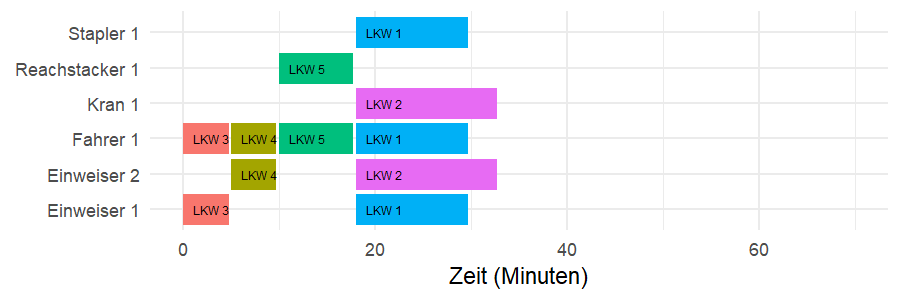
\includegraphics[width=\textwidth]{images/timelines/rsShortestJobNextExample.png}
    \caption{Planung der LKW aus Tabelle \ref{tab:exampleAdvices} nach dem Shortest Job Next Prinzip}
    \label{fig:rsSjnExample}
\end{figure}

Für das gezeigte Beispiel würde das bedeuten, dass diese nach ihrer Bearbeitungsdauer sortiert bearbeitet werden. Zunächst LKW 3 und danach LKW 4, da diese beide den einen verfügbaren Fahrer brauchen und so nicht parallel arbeiten können. LKW 5 kommt anschließend und braucht ebenfalls einen Fahrer. LKW 1 würde dann eingeplant werden, kann aber parallel zu LKW 2 laufen, da hier keine überschneidenden Ressourcen benötigt werden, bzw. es zwei Einweiser gibt.


\textbf{Most Idle Time Next (MIT)}

Ein Hauptziel der Optimierung ist die Reduzierung der Leerlaufzeiten und dadurch eine schnellere und effizientere Abarbeitung der Aufgaben. Eine weitere Idee, um eine möglichst gleichmäßige Auslastung der Ressourcen zu erreichen, wäre es daher, immer den Auftrag als nächstes einzuplanen, der die Ressource mit der bis dahin größten Leerlaufzeit benötigt. Der Gedanke ist hier, dass so eine deutlich gleichmäßigere Auslastung entsteht, da die Aufträge sehr wechselnd verteilt werden. Insgesamt können die Aufgaben so insgesamt potentiell in kürzerer Zeit erledigt werden, da zwischenzeitlich weniger Leerlauf entsteht und alle Ressourcen eine gute Auslastung haben.

\begin{figure}[H]
    \centering
    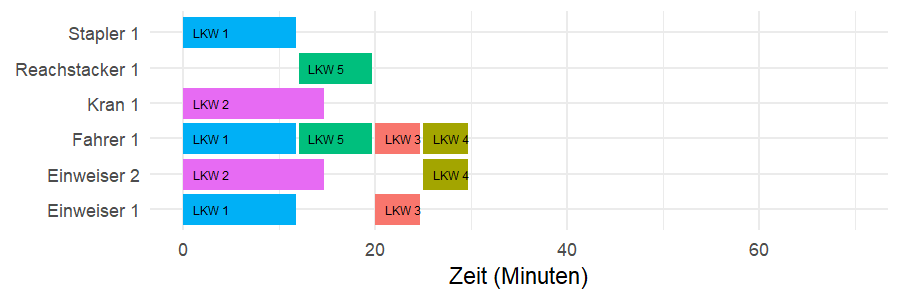
\includegraphics[width=\textwidth]{images/timelines/rsMostIdleExample.png}
    \caption{Planung der LKW aus Tabelle \ref{tab:exampleAdvices} nach dem Most Idle Time Next Prinzip}
    \label{fig:rsMitnExample}
\end{figure}

Für das vorliegende Beispiel  (Abb. \ref{fig:rsMitnExample}) würde dies folgendes bedeuten: Für den Beginn könnte man z.B. nach dem \textit{First Come First Served} Prinzip arbeiten, da sind eben alle Ressourcen noch frei. Anschließend sind Kran und Einweiser noch ganz frei, sodass LKW 2 als nächstes kommen würde. Das gleiche gilt danach für den Reachstacker und LKW 5 und schlussendlich wären dann die Einweiser am wenigsten belegt, sodass LKW 3 und LKW 4 anschließend abgeladen werden.

\textbf{First Come First Served (FCFS)}

Ein letztes Konzept, welches allerdings kein so systematisches Prinzip hat, wäre die Abarbeitung der LKW in der Reihenfolge ihrer Buchung. Theoretisch entsteht dadurch eine nahezu zufällige Reihenfolge. Auch wenn dies im aktuellen, unoptimierten Fall schon sehr ähnlich läuft, wäre hier der Ansatz für Verbesserung, dass das Ganze nun systematisch, mit eine vorgegebenen Zeitplan abläuft. LKW kommen dann eben nicht wann sie wollen. Die der Gedanke ist hier, dass sich dadurch Ungleichheiten ausgleichen und mit Hilfe der Zufallskomponente eine gut durchmischte und gleichmäßige Verteilung entsteht. Bei den anderen Verfahren, insbesondere SJN wäre zu untersuchen, wie gut und gleichmäßig die Verteilung nach solchen Prinzipien wird. Möglicherweise könnten sich Probleme ergeben, dass LKWs gleicher Ladekategorie tendenziell immer kürzer sind und somit viele Ressourcen eines Typs ausgelastet werden, während andere viel Leerlauf behalten.

\begin{figure}[H]
    \centering
    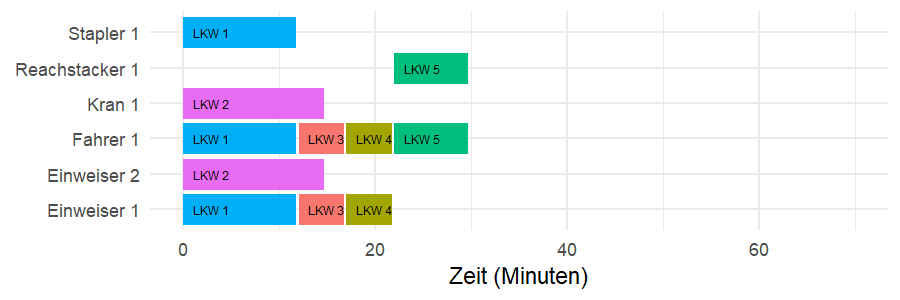
\includegraphics[width=\textwidth]{images/timelines/rsFcfsExample.png}
    \caption{Planung der LKW aus Tabelle \ref{tab:exampleAdvices} nach dem Fist come, first served Prinzip}
    \label{fig:rsFcfsExample}
\end{figure}

Für das hier gezeigte Beispiel (Abb. \ref{fig:rsFcfsExample}) würde dies bedeuten, dass LKW 1 und LKW 2 parallel laufen können und somit schon eine gute Auslastung der Ressourcen in der ersten Zeit ergeben. LKW 3, 4 und 5 müssten dann nacheinander abgearbeitet werden, da alle einen Fahrer benötigen.


\subsubsection{Klassen und Datenstrukturen}
\label{sec:planungRsDatenstrukturen}

Um den zuvor geplanten Algorithmus in Java nachbilden zu können, braucht es einige Klassen und Datenstrukturen, welche implementiert werden sollten. Diese werden an dieser Stelle schon einmal grob geplant, in der späteren Implementierung wird es aber sicherlich noch einige Anpassungen und Erweiterungen geben.

\textbf{Buchungen}

Zum einen wären da die eigentlichen Eingabewerte des Algorithmus, also eine Liste von LKW-Buchungen. Eine entsprechende Klasse soll \textit{TruckAdvice} heißen und muss die folgenden Attribute enthalten:

TruckAdvice
\begin{itemize}
    \item Warentyp (GoodType)
    \item Beschreibung
    \item Anzahl von Packstücken
    \item Handhabungskategorie (HandlingCategory)
    \item Länge, Breite, Höhe der Ladung
    \item Gewicht der Ladung
\end{itemize}

Mögliche Warentypen wurden dabei in der Analyse schon herausgearbeitet. Hier kann eine Enum verwendet werden, um eine erweiterbare Auflistung zu erzeugen. Auch wenn sich die Arbeit hauptsächlich auf Stückgut bezieht, soll die Auswahlmöglichkeit hier dennoch implementiert. Prinzipiell sollte sich dieses Planungssystem nämlich allgemein auf alle Warentypen anwenden lassen, da es nur die Verteilung der Ressourcen übernimmt. Dies kann unabhängig von Warentyp eingestellt werden. So kann einfach direkt der gesamte Prozess im Terminal abgebildet werden.

GoodType
\begin{itemize}
    \item Container
    \item Stückgut
    \item Selbstfahrende Einheit (rollt auf eigener Achse)
    \item Selbstfahrende Einheit (fährt selbstständig herunter)
    \item Nicht selbstfahrende Einheit
\end{itemize}

Die Handhabungskategorie kann ebenfalls über eine erweiterbare Enum abgebildet werden. Hier wurden zunächst die folgenden Optionen aus der Analyse entnommen, mit diesen wird beispielhaft gearbeitet, sicherlich lassen sich hier aber auch noch Erweiterungen finden. 

HandlingCategory
\begin{itemize}
    \item Heben mit Ketten
    \item Heben mit Gabeln
    \item Selbstfahrend
    \item Container
\end{itemize}

\textbf{Zuordnung von Ressourcen}

Um auf den getätigten Buchungen eine Planung aufbauen zu können, muss es eine interne Zuordnung geben, welche zu jeder \textit{HandlingCategory} eine Menge von 
Ressourcen, also Lademaschinen und Hilfsmitteln (\textit{HandlingResource}) zuordnet. Für die Maschinen kann ebenfalls eine Enum verwendet werden, auch hier wurde eine beispielhafte Auswahl verwendet, welche aus der Analyse entnommen wurde. Hier ist auch eine sehr leichte Erweiterung möglich, ohne dass der Algorithmus selbst davon beeinflusst wird. Die Zuordnung der Ressourcen zu den Kategorien kann direkt in der Enum \textit{HandlingCategory} erfolgen, ebenfalls sollte hier pro Kategorie eine Angabe zur Dauer des Ladevorgangs pro Ladegut angegeben werden.

HandlingResource
\begin{itemize}
    \item Gabelstapler
    \item Kran
    \item Reachstacker
    \item Fahrer
    \item Ketten
\end{itemize}


\textbf{Zeitplan}

Das zweite wichtige Datenobjekt für die geplante Implementierung ist der zu erzeugende Zeitplan. Dieses kann prinzipiell relativ simpel aufgebaut werden. Um das Verfahren übersichtlich zu halten, ist die Idee, dass im späteren System ein Zeitplan pro Slot existiert. Dementsprechend soll eine \textit{Schedule}-Klasse erzeugt werden, welche zum einen eine Liste von Ressourcen enthält, welche innerhalb dieses Slot verfügbar sind. Zum anderen muss jeder Ressource eine Liste von Zeiträumen zugeordnet werden, in der diese belegt wird. Die Zeiträume sollen durch eine weitere Klasse \textit{TimeWindow} abgebildet werden. Hier kann Startzeit, Dauer und auch eine Verknüpfung zur jeweiligen Buchung hinterlegt werden. Außerdem braucht ein \textit{Schedule} noch ein Attribut, um die Slotlänge zu hinterlegen.


\textbf{Planungsalgorithmen}

Schlussendlich muss noch die eigentliche Logik, also die Kontrollstrukturen zum erzeugen von Zeitplänen implementiert werden. Um dies erweiterbar zu halten, soll über eine Superklasse eine feste Schnittstelle definiert werden. So kann aus einer Liste von \textit{TruckAdvices} ein \textit{Schedule}-Objekt erzeugt werden. Alle konkreten Algorithmen werden dann in Subklassen davon implementiert und nutzen die identische Schnittstelle. So ist ein leichter Austausch und direkter Vergleich möglich, da alle die gleiche Eingangs- und Ausgangsformate nutzen.


\subsubsection{Vergleichswerte zur Auswertung generieren}
\label{sec:konzeptRsVergleichswerte}

Um eine gute Bewertung der zuvor geplanten Sortierungsverfahren anstellen und eine Verbesserung ermitteln zu können, wäre es von Vorteil, Daten des Ausgangszustands zu haben. Da es allerdings kaum Datensätze gibt, die darstellen würden, wie LKW aktuell verteilt werden, ist die Idee an dieser Stelle, zusätzlich ein Verfahren zu entwickeln, welches einen Zeitplan erzeugen kann, wie es vermutlich im aktuellen und nicht optimierten Zustand erfolgen würde. Dann ließen sich Vorher-Nachher Vergleiche ziehen und eine genauere Bewertung vornehmen.

Ausgangspunkt, wie eine solche Sortierung aussehen würde, ist, dass LKW innerhalb ihres gebuchten Slots kommen, wann sie wollen, d.h. aus Hafensicht gesehen in nahezu zufälliger Reihenfolge. Die Abarbeitung würde also nach dem \glqq{}first come, first served\grqq{} Prinzip erfolgen. Erschwerend kommt allerdings noch hinzu, dass die LKW wie erwähnt nicht alle direkt bereit stehen, sondern zusätzlich noch zu einem aus Hafensicht zufälligen Zeitpunkt erscheinen, wodurch eine sehr lückenhafte Verteilung mit vielen Leerlaufzeiten der Ressourcen entsteht. Um diesen Sachverhalt zu implementieren ist es also die Idee, sowohl die Reihenfolge der LKW Buchungen, als auch jeweils einen Ankunftszeitpunkt innerhalb des Slots zufällig zu bestimmen. Anschließend kann jeder LKW zu seinen benötigten Ressourcen zugeteilt werden, entweder sobald er ankommt oder spätestens, wenn alle von ihm benötigten Ressourcen verfügbar sind. Auch dieses Verfahren soll in der prototypischen Umsetzung implementiert und integriert werden.


\subsection{Konzeption Algorithmus 2}

Wie auch schon Variante 1, soll auch dieser Prototyp in Java umgesetzt werden. Auch hier geht es hauptsächlich darum, die Algorithmen und Hintergrundlogik zu implementieren und weniger darum, schöne Benutzeroberflächen für direkte Benutzerein- und ausgaben zu schaffen. Auch die Erfassung der Daten von Fahrern und Speditionen soll nicht Teil er Implementierung sein, also auch nicht die Sammlung von Buchungen für die Slots o.ä. Stattdessen erfolgt der Aufruf der Algorithmen über JUnit Testfälle. Hier soll mit gezielten oder generierten Eingabedaten gearbeitet werden und damit die Optimierung entsprechend durchgeführt werden.

\subsubsection{Klassen und Datenstrukturen}

Die benötigten Datenstrukturen sind dabei sehr vergleichbar zu denen, die für den anderen Algorithmus geplant wurden. Die Details zu Attributen und Enums können also aus dieser Planung in Kapitel \ref{sec:planungRsDatenstrukturen} übernommen werden. Der wichtigste Unterschied liegt dabei intern bei der Zuordnung der benötigten Ressourcen zu den \textit{HandlingCategories}. Einer Kategorie ist hier direkt eine Maschine zugeordnet, welche repräsentativ für alle hier benötigten Ressourcen steht. Der Fokus wurde in diesem Fall auf die Zeitaufwände bei der Bearbeitung gelegt. Zu jeder Maschine werden deshalb in diesem Projekt neben der bereits bekannten Bearbeitungszeit pro Ladegut zusätzlich noch die benötigten Zeiten für Auf- und Abbau hinterlegt. 


\subsubsection{Ablauf}

Das grundsätzliche Verfahren, nachdem eine Liste aller Buchungen (also die Liste von \textit{TruckAdvice}-Objekten) erfasst wurde, ist in Abbildung \ref{fig:flowchart_tsp_algorithm} dargestellt. Alle blauen Kästen stellen dabei die hier betrachteten und direkt implementierten Bestandteile dar. Um eine Eingabe in das Traveling Salesman Problem zu überführen, muss ein entsprechender Graph erzeugt werden. Auch dazu wird es noch eine passende Datenstruktur zu internen Repräsentation geben müssen, welche allerdings sehr von der Implementierung der weiterer Lösungsverfahren abhängt und daher noch nicht genauer geplant wurde. Die Lösung des TSP ist damit auch schon der zweite Schritt der Prozesskette. Dieser Baustein soll austauschbar gestaltet werden, sodass hier verschiedene Verfahren implementiert und getestet werden können. Schlussendlich muss die daraus ermittelte Reihenfolge wieder in einen einheitlichen Zeitplan überführt werden. Es soll dann also eine zu Algorithmus 1 vergleichbare Darstellung geben, in der die jeweiligen Ladeplätze gespeichert sind und wo es eine entsprechende Zuordnung und Reihenfolge der Buchungen zu den Ladeplätzen gibt.

\begin{figure}[H]
    \centering
    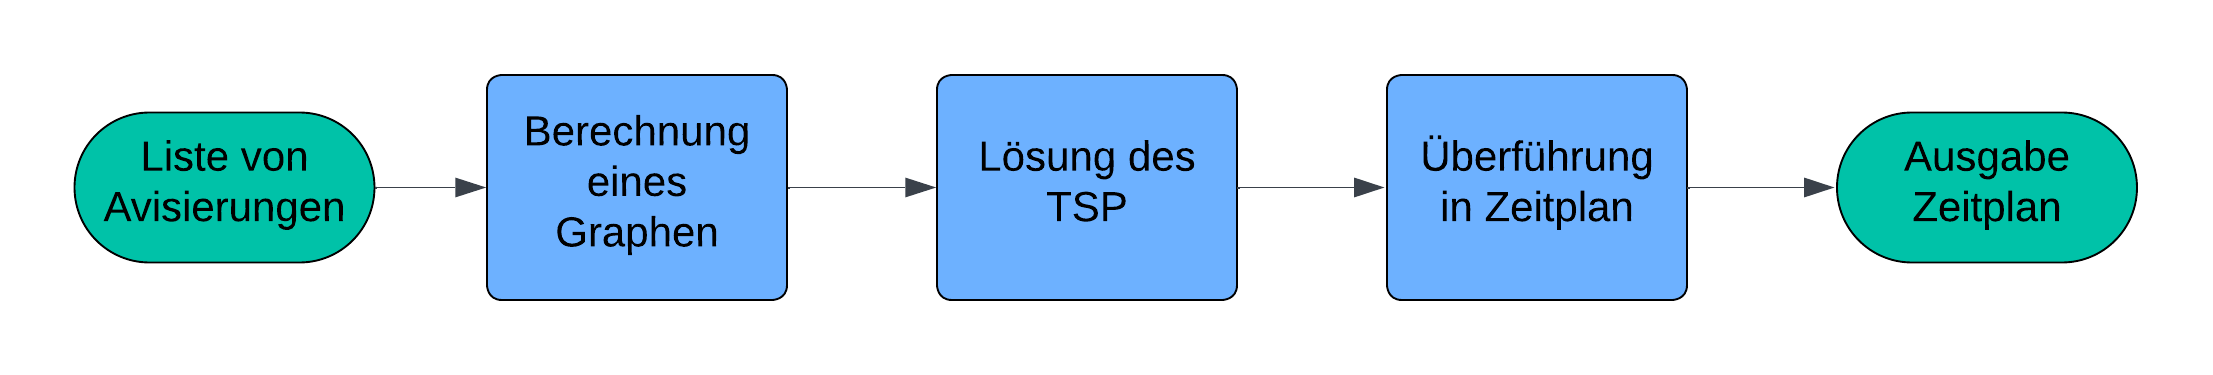
\includegraphics[width=\textwidth]{images/Flowchart TSP Algorithm.png}
    \caption{Ablaufdiagramm der Lösung mittels TSP}
    \label{fig:flowchart_tsp_algorithm}
\end{figure}

Detailliertre Planungen zu den einzelnen Bausteinen dieses Ablaufs wurden in den hier folgenden Kapiteln geplant.

\subsubsection{Berechnung eines Graphen}
\label{sec:berechnungGraphenTsp}

Zunächst einmal kann aus den gegebenen Daten ein vollständiger, gerichteter Graph erzeugt werden. In der Implementierung kann dieser auch als zweidimentionale Matrix dargestellt werden. Dabei ist jeder Knoten ein Auftrag aus der eingegebenen Liste. Für die Kanten wird eine Methode benötigt, die die Kosten bzw. Aufwände berechnen kann, welche benötigt werden, um einen beliebigen LKW nach einem Anderen abzufertigen. Um eine vergleichbare Einheit zu haben, wird hier immer mit Zeit in Minuten gearbeitet. Aus der bei der Datenerfassung ermittelten \textit{HandlingCategory} kann jeweils bestimmt werden, welche Ladehilfsmittel (\textit{HandlingMachine}) und Ressourcen benötigt werden. Zu jedem Hilfsmittel sind in dem System entsprechende Zeiten hinterlegt. Für das hier zu erstellende Proof of Concept sollen das zunächst Anfahrt-/Aufbauzeit, Abbau./Abfahrtszeit und Ladezeit pro Gut sein. Denkbar wären hier allerdings auch deutlich komplexere Berechnungen und Einflussfaktoren. Beispielsweise unterschiedliche Wechselaufwände, je nachdem zu welcher Maschine gewechselt wird. Um die Komplexität an dieser Stelle nicht zu hoch werden zu lassen, werden die Kosten zum Abfertigen von LKW B nach LKW A nach folgendem Schema berechnet:

Gleiche Maschine für A und B?\\
\begin{equation} \label{eq:tspCost1}
    Zeit_{AB} = numberOfGoods_B * ZeitProGut_B
\end{equation}

Ist ein Wechsel der Maschine nötig?\\
\begin{equation} \label{eq:tspCost2}
    Zeit_{AB} = Abbauzeit_A + Aufbauzeit_B + numberOfGoods_B * ZeitProGut_B
\end{equation}

Ein so erzeugter Graph bzw. dessen interne Darstellung als Matrix könnten wie in den Abbildungen \ref{fig:example_tsp_graph} und \ref{fig:example_tsp_matrix} aussehen.

\begin{figure}[H]
\centering
\begin{minipage}{.6\textwidth}
  \centering
  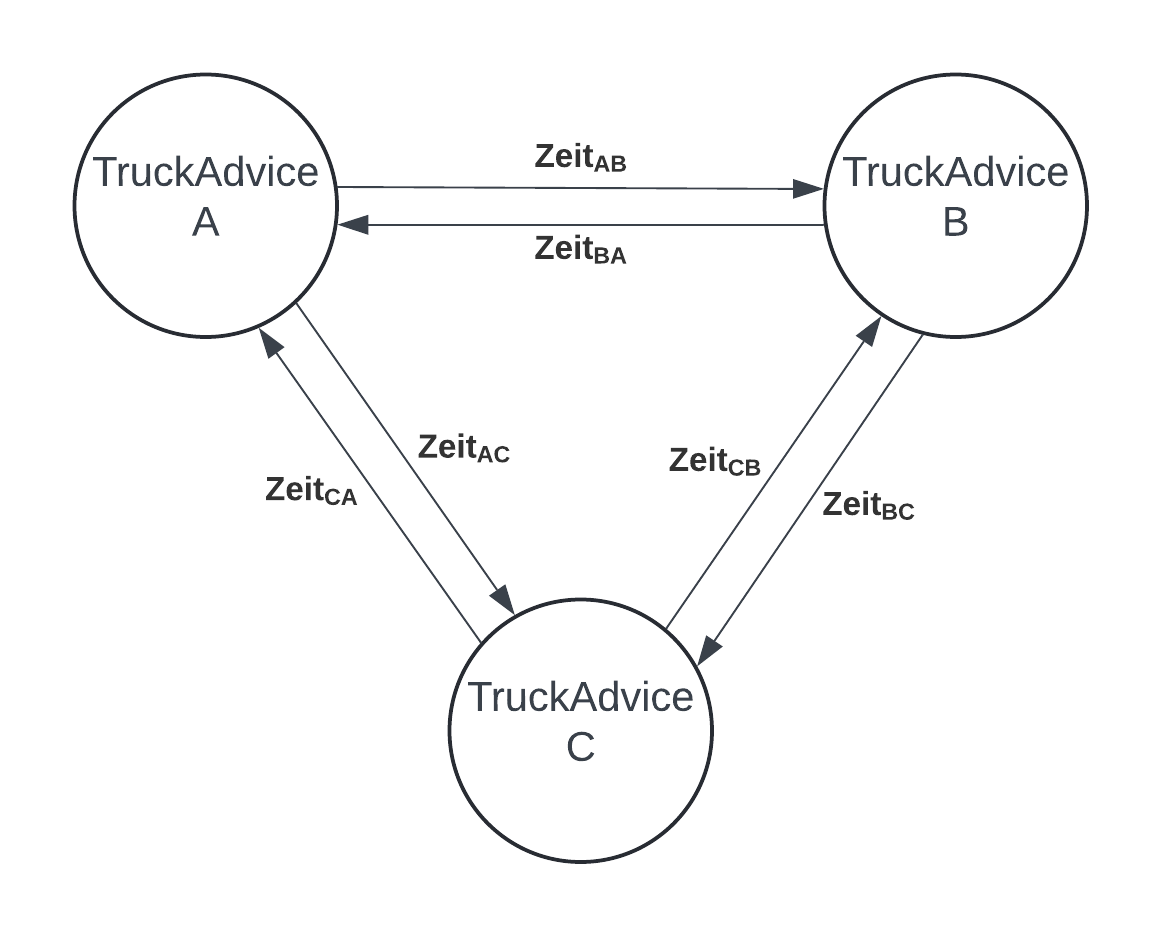
\includegraphics[width=\linewidth]{images/ExampleTSPGraph.png}
  \caption{Beispielhafte Darstellung von TruckAdvices mit Zeitaufwänden als Graph}
  \label{fig:example_tsp_graph}
\end{minipage}%
\begin{minipage}{.4\textwidth}
  \centering
    \[
    \begin{matrix}
         & A & B & C\\
        A & \infty & Zeit_{AB} & Zeit_{AC}\\
        B & Zeit_{BA} & \infty & Zeit_{BC}\\
        C & Zeit_{CA} & Zeit_{CB} & \infty
    \end{matrix}
    \]
  \caption{Zu Abb. \ref{fig:example_tsp_graph} passende Matrix}
  \label{fig:example_tsp_matrix}
\end{minipage}
\end{figure}
\todo{Matrix als Abb bezeichnen ok? evtl ändern...}



\subsubsection{TSP Lösungsverfahren}
\label{sec:tspVerfahrenPlanung}
\todo{Problem: Sehr unterschiedlich lange Zeit je Slot erwähnen und Lösung beschreiben}

Der zweite und wesentliche Schritt zur Optimierung ist nun die Lösung des TSP, also das Finden eines möglichst kurzen Weges durch den zuvor erzeugten Graphen. Mit Blick auf das zu erzielende Ergebnis fällt auf, dass das nach dem standardmäßigen TSP für einen Handlungsreisenden eine Kette von Stationen erzeugt würde. Übertragen auf das vorliegende Problem heißt das, dass aus allen Buchungen ein Zeitplan für einen einzigen Ladeplatz erzeugt wird. Dies ist zunächst auch ein gutes Zwischenergebnis und erfüllt schon einmal viele zuvor gesetzten Anforderungen. Um allerdings ein praxisnäheres Szenario abzubilden, wäre die Erweiterung auf mehrere Ladeplätze ein nicht ganz uninteressanter Punkt, um diesen hier bei der Planung ebenfalls umzusetzen. Dies ist bei genauerer Auseinandersetzung mit dem TSP und dessen Varianten auf den ersten Blick kein allzu großes Problem mehr. Für diesen Anwendungsfall dürfte nämlich das mTSP\todo{mtsp erstes mal erwähnt? evtl hier ausschreiben} geeignet sein \cite{mtsp}. Hier werden statt einem Handlungsreisenden mehrere auf das gleiche Szenario angesetzt, die dann die Stationen unter sich aufteilen und parallel abarbeiten können. Dadurch ist die Vorarbeit die selbe, nur dass über die Anzahl von Handlungsreisenden nun entschieden werden kann, für wie viele Ladeplätze die Optimierung erfolgen soll.

Rein aus dieser theoretischen Sicht ist das TSP bzw. mTSP gar nicht so schwer zu verstehen und auf das vorliegende Problem zu übertragen. Für die Implementierung dieses wesentlichen Lösungsschrittes aus dem Ablaufdiagramm (Abb. \ref{fig:flowchart_tsp_algorithm}), müssen nun allerdings passende Lösungsverfahren gefunden werden. Hier lassen sich für das normale TSP auch noch überschaubare Verfahren finden. Sehr viel komplizierter wird es bei der Lösung des mTSP. Hier sind die Verfahren sehr viel komplexer und schwieriger. Nach einiger Recherche hat sich die  Überführung eines mTSP in ein gewöhnliches TSP als noch überschaubar und vom Aufwand her umsetzbar dargestellt. Dies hat den sehr großen Vorteil, dass zur Findung des besten Weges anschließend die ganz normalen, bekannteren und einfacheren Verfahren zur Lösung von TSP genutzt werden können. Der übersichtlichkeit halber wird diese Transofrmation im nächsten Kapitel \ref{sec:mstpTransofrmation}\todo{Vorwärtsverweis erlaubt?} genauer erläutert. \cite{mtsp, mtspAlgosAndTransform}


Aus Softwaresicht muss nun also ein passendes Verfahren zur Lösung des TSP implementiert werden. Da Quellen mit passenden Implementierungen gefunden wurden, soll eine manuelle Implementierung, ohne Libraries erfolgen. Gleichzeitig lässt sich so eine bessere Kontrolle und Anpassbarkeit auf das vorliegende Problem erzielen und auch die Verfahren sind so besser verständlich. Da es einige verschiedene Algorithmen und Ansätze zur Lösung gibt, sollen hier mehrere implementiert werden, um diese anschließend zu vergleichen. Die nachfolgende Auswahl beschreibt die bekanntesten Methoden und erklärt, welche es sich potentiell lohnt umzusetzen, da das Verhältnis zwischen Aufwand der Implementierung und Qualität des Ergebnisses am besten erscheint.

\textbf{Brute-Force Methode}

Zum einen sollen hier exakte Verfahren betrachtet werden. Der ineffizienteste und aufwändigste Weg, ist die \textit{brute-force Methode}, d.h. alle möglichen Lösungswege durchgehen, deren Länge berechnen und immer wieder schauen, ob ein kürzerer gefunden wurde. Die Implementierung wäre vermutlich nicht allzu kompliziert, allerdings wird diese Methode sehr schnell an ihre Leistungsgrenze kommen. Da es hier wirklich offensichtlich bessere Ansätze gibt, wird dieser Weg aber nicht weiter verfolgt und wurde hier nur der Vollständigkeit halber erwähnt. \cite{oracleTsp}

\textbf{Branch and Bound} \todo{potentielle Grenzen in Literatur erwähnt, also max Anzahl möglicher Knoten?}
\todo{Beschreibung/Erklärung in Quelle \cite{constraintProgramming}, Seriöse Quellen hinzufügen, evtl. erweitern und überarbeiten}

Besser geeignet erscheint dagegen das \textit{Branch and Bound Verfahren}. Von der Grundidee ist dieses sehr ähnlich zum brute-forcing, allerdings kann hier über spezielle Verfahren direkt die Länge des kürzest möglichen Wegs berechnet. Anschließend können dann per Ausschlussverfahren schon frühzeitig einige längere Wege ausgeschlossen werden, sodass der Gesamtaufwand der Berechnung verkürzt wird. \cite{travelingSalesman}

Das Prinzip dabei ist es, für jeden betrachteten Knoten eine \glqq{}Bound\grqq{}, also Grenze für einen Wert für die bestmögliche Lösung beim Weiterverfolgen der angrenzenden Knoten. Anhand dessen kann dann beim Durchgehen der Äste und Möglichkeiten des Graphen entschieden werden, ob es sich im Vergleich zur insgesamt besten Lösung lohnt, die vorliegende Option weiter zu verfolgen oder ob diese bereits jetzt zu teuer ist und verworfen werden kann. Die minimalen Kosten können dabei berechnet werden, indem von allen Knoten die Kosten der kleinsten Kante und die der zweitkleinsten Kante summiert werden und das Gesamtergebnis halbiert wird. Die Halbierung wird vorgenommen, da jede Kante zweimal vorkommt. \cite{geeksForGeeksBnB}

\textbf{Reduced Matrix} \todo{potentielle Grenzen in Literatur erwähnt, also max Anzahl möglicher Knoten?}

Ein weiteres interessantes und exaktes Verfahren ist die \textit{Reduced Matrix Methode}. Diese ähnelt sehr dem Prinzip des Branch and Bound Ansatzes, hierbei wird die optimale Lösung allerdings rechnerisch über die Umformung von Matrizen ermittelt. 

Das Prinzip ist es hier, dass die Zeilen und Spalten der Kostenmatrix reduziert werden können. Es wird dafür Zeile für Zeile und anschließend Spalte für Spalte durchgegangen. Enthalten diese jeweils keinen 0-Wert, so kann von allen Werten der jeweils kleinste abgezogen werden. Summiert man die Werte jeder Zeile und jeder Spalte, welche reduziert wurden, so ergeben sich die minimalen Kosten für diesen (Teil-)Graphen. \cite{geeksForGeeksRm}

\begin{figure}[H]
\centering
\begin{minipage}{.5\textwidth}
  \centering
  \[
    \begin{matrix}
          & 1 & 2 & 3 & 4\\
        1 & \infty & 10 & 15 & 20\\
        2 & 10 & \infty & 35 & 25\\
        3 & 15 & 35 & \infty & 30\\
        4 & 20 & 25 & 30 & \infty\\
    \end{matrix}
    \]
    \caption{Initiale Matrix \cite{geeksForGeeksRm}}
    \label{fig:reduced_matrix_initial}
\end{minipage}%
\begin{minipage}{.5\textwidth}
  \centering
   \[
    \begin{matrix}
          & 1 & 2 & 3 & 4\\
        1 & \infty & 0 & 5 & 10\\
        2 & 0 & \infty & 25 & 15\\
        3 & 0 & 20 & \infty & 15\\
        4 & 0 & 5 & 10 & \infty\\
    \end{matrix}
    \]
    \caption{Reduzierte Matrix aus Abb. \ref{fig:reduced_matrix_initial} \cite{geeksForGeeksRm}}
    \label{fig:reduced_matrix_reduced}
\end{minipage}
\end{figure}

Die Zeilen aus Abbildung \ref{fig:reduced_matrix_initial} wurden jeweils um 10, 10, 15, 20 reduziert und die Spalten dann um 0, 0, 5, 10. So ergibt sich minimale Kosten für den gesamten Graphen von 10 + 10 + 15 + 20 + 5 + 10 = 70. Um im Baum fortzuschreiten kann die Matrix anschließend für jede Kante weiter reduziert werden. Um beispielsweise von Knoten 1 zu 2 zu kommen, werden die Werte der ersten Zeile und zweiten Spalte durch unendlich ersetzt und die Matrix erneut reduziert (siehe Abb. \ref{fig:reduced_matrix_1-2}). 

\begin{figure}[H]
\centering
\begin{minipage}{.5\textwidth}
  \centering
  \[
    \begin{matrix}
          & 1 & 2 & 3 & 4\\
        1 & \infty & \infty & \infty & \infty\\
        2 & 10 & \infty & 35 & 25\\
        3 & 15 & \infty & \infty & 30\\
        4 & 20 & \infty & 30 & \infty\\
    \end{matrix}
    \]
    \caption{Matrix des Schritts von Knoten 1 zu Knoten 2 \cite{geeksForGeeksRm}}
    \label{fig:reduced_matrix_1-2}
\end{minipage}%
\begin{minipage}{.5\textwidth}
  \centering
   \[
    \begin{matrix}
          & 1 & 2 & 3 & 4\\
        1 & \infty & \infty & \infty & \infty\\
        2 & 0 & \infty & 10 & 0\\
        3 & 0 & \infty & \infty & 5\\
        4 & 0 & \infty & 0 & \infty\\
    \end{matrix}
    \]
    \caption{Reduzierte Matrix aus Abb. \ref{fig:reduced_matrix_1-2} \cite{geeksForGeeksRm}}
    \label{fig:reduced_matrix_1-2_reduced}
\end{minipage}
\end{figure}


Hier wird um 5, 0 und 0 bzw. um 0, 5 und 0 reduziert. Die Kosten der Reduktion von 10 können dann auf die zuvor ermittelten 70 addiert werden, um die minimalen Kosten im Baum zu erhalten.


So lässt sich aus dem beispielhaften Graphen in Abbildung \ref{fig:reducedMatrixGraph} im Endeffekt der Baum aus Abbildung \ref{fig:reducedMatrixTree} bestimmen. Einige Äste mussten dabei nicht weiter verfolgt werden, da sie schon zum betrachteten Zeitpunkt nicht weniger Kosten würden als andere. Es zeigt sich, dass die Wege 1\textgreater{}3\textgreater{}4\textgreater{}2 und 1\textgreater{}2\textgreater{}4\textgreater{}3 die kürzesten sind. Zum Vorteil wird hier auch ausgenutzt, dass für das TSP immer geschlossene Pfade gesucht werden, d.h. hier ist es irrelevant mit welchem Knoten begonnen wird, es kann einfach mit einem beliebigen Knoten, in diesem Fall Knoten 1 gestartet werden. \cite{geeksForGeeksRm}

\begin{figure}[H]
\centering
\begin{minipage}{.4\textwidth}
  \centering

    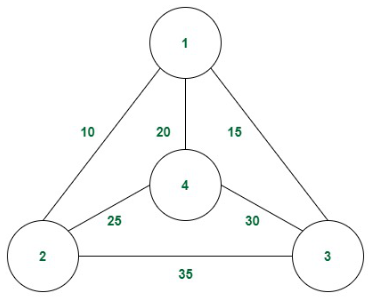
\includegraphics[width=\textwidth]{images/reducedMatrixGraph.png}
    \caption{Beispielhafter Graph}
    \label{fig:reducedMatrixGraph}

\end{minipage}%
\begin{minipage}{.6\textwidth}
  \centering
    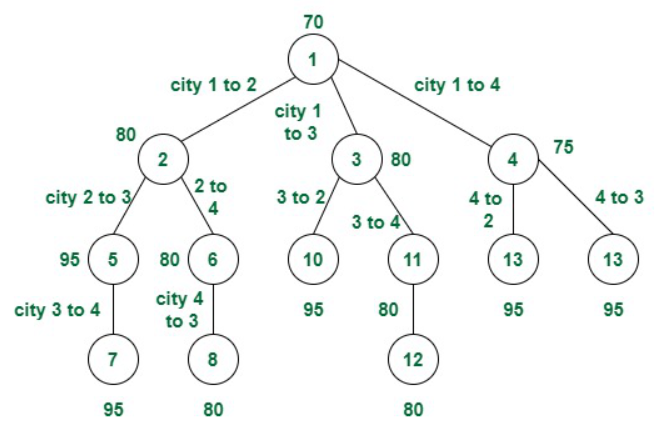
\includegraphics[width=\textwidth]{images/reducedMatrixTree.png}
    \caption{Alle mit der Reduced Matrix Methode betrachteten Pfade}
    \label{fig:reducedMatrixTree}
\end{minipage}
\end{figure}


\textbf{Simulated Annealing}

Ein weiterer Blick lohnt sich allerdings auch auf die heuristischen Verfahren. Im Gegensatz zu den zuvor beschriebenen, exakten Varianten, wird es hier nicht garantiert das beste Ergebnis geben. Allerdings wird es in den meisten Fällen dem besten Ergebnis sehr nahe kommen. Der große Vorteil könnte dafür allerdings sein, dass die Rechenzeit deutlich verringert wird. Dies könnte vor allem ein wichtiger Kompromiss sein, da die Größe der durch die anderen Verfahren lösbaren Graphen sehr begrenzt sein wird, gerade mit überschaubaren Rechenressourcen. Mit dem \textit{Simulated Annealing Ansatz} sollte der Rechnenaufwand um ein vielfaches geringer sein und damit auch die Größe von möglichen Graphen deutlich steigen. \cite{tspSimulatedAnnealing}

Dieses Verfahren macht sich zu nutze, dass man sich den Aufwand für jede Wegkombination im Graphen des TSP als kontinuierliche Funktion vorstellen kann. Ziel ist es dabei grundsätzlich das globale Optimum, also den kleinsten Wert über alle Möglichkeiten zu finden. Im Gegensatz zu den vorherigen Varianten, welche alle Möglichkeiten durchgehen, ist hier die Idee, sich dem besten Ergebnis durch ausprobieren bestimmter Möglichkeiten anzunähern. Dabei fängt man mit einer zufälligen Reihenfolge an. Nach jedem Versuch führt man kann man unterschiedliche, zufällige Operationen an der Reihenfolge durchführen, u.a. Tauschen von zwei Knoten oder Verschieben eines Knotens. Auch die Nutzung von 2-Opt oder 3-Opt-Heuristiken ist denkbar. Hier werden zwei oder drei Kanten zwischen Knoten getrennt und untereinander neu verbunden, sodass sich einer neuer Pfad ergibt. Durch erneute Berechnung des Aufwand kann nun geschaut werden, ob sich das Ergebnis verbessert hat, dann wird dies als neuer Ausgangspunkt genutzt, andernfalls wird es verworfen. Durch Wiederholung dieses Vorgangs sollte sich das Ergebnis einem Optimum annähern. Es kann allerdings sein, dass dies ein lokales und kein globales Optimum ist. Hier kommt der eigentliche Trick des Simulated Annealings ins Spiel, es wird mit einer \glqq{}Temperatur\grqq{} gearbeitet. Durch eine exponentielle Funktion wird unter bestimmten Umständen doch das schlechtere Ergebnis gespeichert und die Möglichkeit geschaffen, aus dem lokalen Optimum auszubrechen. Durch senken der Temperatur im Verlauf der versuche wird diese Wahrscheinlichkeit geringer. Dieses Verfahren hat man sich von Abkühlungsprozessen aus der Natur abgeschaut. \cite{tspSimulatedAnnealing}

\begin{figure}[H]
    \centering
    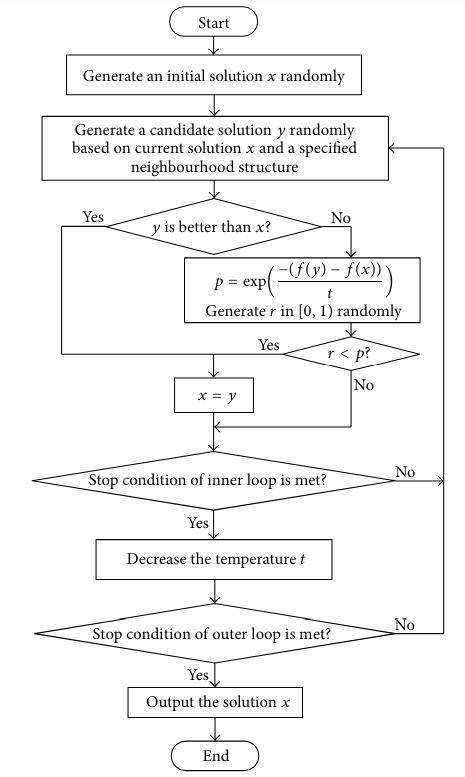
\includegraphics[width=0.6\textwidth]{images/flowSimulatedAnnealing.png}
    \caption{Ablauf von Simulated Annealing \cite{tspSimulatedAnnealing}}
    \label{fig:flowchart_simulated_annealing}
\end{figure}

Der schematische Ablauf eines Simulated Annealing Prozesses ist in Abbildung \ref{fig:flowchart_simulated_annealing} dargestellt. Der Nachteil dieses Verfahrens ist, dass es mehrere Parameter gibt, die eingestellt werden müssen. So gibt es eine Maximalanzahl von Schleifendurchläufen, eine Starttemperatur und eine Abkühlungsrate. All diese Werte beeinflussen das Ergebnis. Komplexere Implementierungen können diese Werte selbst anpassen, eine manuelle Einstellung ist oft nicht so einfach und passiert eher nach dem \glqq{}trail and error\grqq{}-Prinzip. \cite{tspSimulatedAnnealing}

Insgesamt scheint die diese Variante zur Lösung allerdings vielversprechende Ergebnisse zu liefern und auch keine allzu komplexe Implementierung darzustellen. Auch dieses Verfahren soll deshalb neben den beiden zuvor beschriebenen, exakten Verfahren implementiert werden. Zum einen kann so ein direkter Vergleich zwischen exakten und heuristischen Ansätzen durchgeführt werden. Zum anderen ist dies aber auch die potentiell beste Lösung für besonders große Graphen und kann dort eigesetzt werden, wo die anderen Verfahren ihre Grenze erreichen.


\subsubsection{Transformation eines mTSP zu einem TSP}
\label{sec:mstpTransofrmation}

Um ein mTSP in ein einfaches TSP umzuwandeln, fügt man dem Graphen fiktive Knoten für die Startpunkte der Handlungsreisenden hinzu. Für ein beispielhaftes Problem aus n=9 Knoten und m=2 Handlungsreisenden fügt man m-1, also noch einen fiktiven Knoten hinzu. Ein Knoten wird ebenfalls fest als Startpunkt eines Handelsreisenden definiert. Das genannte Beispiel ist in Abbildung \ref{fig:mtsp_tranformation} zu sehen, wobei Knoten 1 der definierte Startpunkt und Knoten 10 der hinzugefügte, fiktive Knoten ist. Wie im Vergleich der Ausgangsmatrix (Abbildung \ref{fig:mtsp_distance_matrix}) und der erweiterten Maxtrix (Abbildung \ref{fig:mtsp_distance_matrix_with_dummys}) zu sehen ist, werden die Gewichte zwischen den Startpunkten sehr hoch gesetzt, wie es auch schon in der Diagonalen zwischen identischen Knoten der Fall ist, sodass keine Reisen direkt zwischen Startpunkten möglich ist. Ein Nachteil ist allerdings, dass die Größe des Graphen bzw. der Matrix ansteigt und dadurch der Lösungsaufwand erhöht wird, welcher mit steigender Zahl von Knoten ohnehin schon exponentiell steigt. \cite{mtsp, mtspTransform2}

\begin{figure}[H]
    \centering
    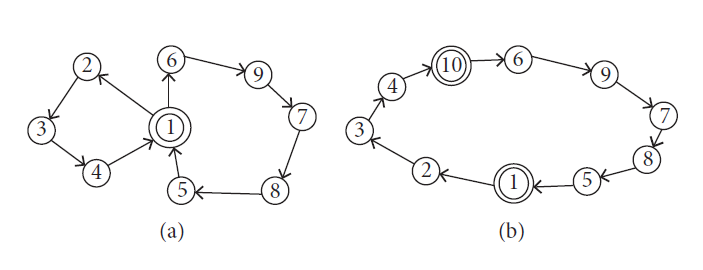
\includegraphics[width=\textwidth]{images/mtspTransformation.png}
    \caption{Lösung eines mTSP und Transformation zu TSP \cite{mtspTransform2}}
    \label{fig:mtsp_tranformation}
\end{figure}

\setcounter{MaxMatrixCols}{20}
\begin{figure}[H]
\centering
\begin{subfigure}{.44\textwidth}
  \centering
  \begin{footnotesize}
    \[
    \setlength{\arraycolsep}{0.1cm}
    \begin{matrix}
          & 1 & 2 & 3 & 4 & 5 & 6 & 7 & 8 & 9\\
        1 & 999 & 7 & 15 & 9 & 10 & 6 & 8 & 9 & 10\\
        2 & 11 & 999 & 8 & 7 & 11 & 3 & 6 & 4 & 3\\
        3 & 15 & 5 & 999 & 16 & 12 & 5 & 8 & 13 & 4\\
        4 & 2 & 5 & 11 & 999 & 9 & 13 & 14 & 4 & 2\\
        5 & 8 & 6 & 3 & 5 & 999 & 6 & 7 & 10 & 9\\
        6 & 6 & 13 & 8 & 11 & 5 & 999 & 5 & 4 & 5\\
        7 & 5 & 15 & 3 & 7 & 12 & 6 & 999 & 8 & 9\\
        8 & 9 & 3 & 9 & 14 & 3 & 11 & 8 & 999 & 10\\
        9 & 11 & 16 & 3 & 9 & 10 & 7 & 9 & 10 & 999\\
        &&&&&&&&&
    \end{matrix}
    \]
    \end{footnotesize}
  \caption{Distanzmatrix}
  \label{fig:mtsp_distance_matrix}
\end{subfigure}
\begin{subfigure}{.54\textwidth}
  \centering
  \begin{footnotesize}
  \[
  \setlength{\arraycolsep}{0.1cm}
    \begin{matrix}
          & 1 & 2 & 3 & 4 & 5 & 6 & 7 & 8 & 9 & 10\\
        1 & 999 & 7 & 15 & 9 & 10 & 6 & 8 & 9 & 10 & 999\\
        2 & 11 & 999 & 8 & 7 & 11 & 3 & 6 & 4 & 3 & 11\\
        3 & 15 & 5 & 999 & 16 & 12 & 5 & 8 & 13 & 4 & 15\\
        4 & 2 & 5 & 11 & 999 & 9 & 13 & 14 & 4 & 2 & 2\\
        5 & 8 & 6 & 3 & 5 & 999 & 6 & 7 & 10 & 9 & 8\\
        6 & 6 & 13 & 8 & 11 & 5 & 999 & 5 & 4 & 5 & 6\\
        7 & 5 & 15 & 3 & 7 & 12 & 6 & 999 & 8 & 9 & 5\\
        8 & 9 & 3 & 9 & 14 & 3 & 11 & 8 & 999 & 10 & 9\\
        9 & 11 & 16 & 3 & 9 & 10 & 7 & 9 & 10 & 999 & 11\\
        10 & 999 & 7 & 15 & 9 & 10 & 6 & 8 & 9 & 10 & 999\\
    \end{matrix}
    \]
    \end{footnotesize}
  \caption{Erweiterte Distanzmatrix}
  \label{fig:mtsp_distance_matrix_with_dummys}
\end{subfigure}

\caption{Distanzmatrixen zum Beispiel in Abb. \ref{fig:mtsp_tranformation} \cite{mtspTransform2}}
\label{fig:mtspMatricies}
\end{figure}

\begin{comment}

\begin{figure}[H]
    \centering
    \begin{small}
    \[
    \begin{matrix}
          & 1 & 2 & 3 & 4 & 5 & 6 & 7 & 8 & 9\\
        1 & 999 & 7 & 15 & 9 & 10 & 6 & 8 & 9 & 10\\
        2 & 11 & 999 & 8 & 7 & 11 & 3 & 6 & 4 & 3\\
        3 & 15 & 5 & 999 & 16 & 12 & 5 & 8 & 13 & 4\\
        4 & 2 & 5 & 11 & 999 & 9 & 13 & 14 & 4 & 2\\
        5 & 8 & 6 & 3 & 5 & 999 & 6 & 7 & 10 & 9\\
        6 & 6 & 13 & 8 & 11 & 5 & 999 & 5 & 4 & 5\\
        7 & 5 & 15 & 3 & 7 & 12 & 6 & 999 & 8 & 9\\
        8 & 9 & 3 & 9 & 14 & 3 & 11 & 8 & 999 & 10\\
        9 & 11 & 16 & 3 & 9 & 10 & 7 & 9 & 10 & 999
    \end{matrix}
    \]
    \end{small}
    \caption{Distanzmatrix des mTSP Beispiels \cite{mtspTransform2}}
    \label{fig:mtsp_distance_matrix}
\end{figure}

\begin{figure}[H]
    \centering
    \[
    \begin{matrix}
          & 1 & 2 & 3 & 4 & 5 & 6 & 7 & 8 & 9 & 10\\
        1 & 999 & 7 & 15 & 9 & 10 & 6 & 8 & 9 & 10 & 999\\
        2 & 11 & 999 & 8 & 7 & 11 & 3 & 6 & 4 & 3 & 11\\
        3 & 15 & 5 & 999 & 16 & 12 & 5 & 8 & 13 & 4 & 15\\
        4 & 2 & 5 & 11 & 999 & 9 & 13 & 14 & 4 & 2 & 2\\
        5 & 8 & 6 & 3 & 5 & 999 & 6 & 7 & 10 & 9 & 8\\
        6 & 6 & 13 & 8 & 11 & 5 & 999 & 5 & 4 & 5 & 6\\
        7 & 5 & 15 & 3 & 7 & 12 & 6 & 999 & 8 & 9 & 5\\
        8 & 9 & 3 & 9 & 14 & 3 & 11 & 8 & 999 & 10 & 9\\
        9 & 11 & 16 & 3 & 9 & 10 & 7 & 9 & 10 & 999 & 11\\
        10 & 999 & 7 & 15 & 9 & 10 & 6 & 8 & 9 & 10 & 999\\
    \end{matrix}
    \]
  \caption{Erweiterte Distanzmatrix aus Abb. \ref{fig:mtsp_distance_matrix}  \cite{mtspTransform2}}
  \label{fig:mtsp_distance_matrix_with_dummys}
\end{figure}

\end{comment}

\subsubsection{Umwandlung der TSP Lösung in einen Zeitplan}
\label{sec:tspToSchedule}

Nachdem ein nun also eine Reihenfolge gefunden wurde, in der die LKW sich am schnellsten bearbeiten lassen, muss daraus ein Zeitplan erstellt werden. Da es bereits eine Methode gibt, um die Zeiten zwischen den LKW zu berechnen, ist es nicht mehr schwierig, jeweils die Zeitpunkte zu bestimmen, in denen jeder LKW am Terminal erscheinen muss.

Eine Herausforderung, die sich bei der Planung für mehrere Ladeplätze mittels mTSP ergeben wird, ist, dass dieses Verfahren zwar die kürzeste Gesamtzeit berechnet, die Anzahl der Aufträge bzw. der Zeitaufwand pro Ladeplatz wird allerdings nicht unbedingt gleichmäßig verteilt sein. Es wird oft der Fall sein, dass ein Ladeplatz deutlich mehr Zeit benötigt, als ein Anderer. Hinzu kommt, dass nicht unbedingt gewährleistet ist, dass alle Buchungen, die für einen Slot aufgenommen wurden auch in diesen hinein passen. Ein Beispielzeitplan, wie er möglicherweise durch die Lösung des mTSP erzeugt wird, ist in Abbildung \ref{fig:tspCutExample1} zu sehen. Dafür wurde ein Ansatz zur Lösung erdacht, welcher die über das Slotende hinausragenden Zeiträume abzuschneiden und auf eventuelle Lücken verteilen soll. Dadurch wird sich die Gesamtdauer der Abfertigung sicherlich verschlechtern und die Reihenfolge wird nicht mehr ganz optimal sein, dennoch ist dies besser als große, gänzlich ungenutzt Zeiträume bei einigen Ladeplätzen zu haben und an anderer Stelle LKW komplett wegfallen lassen zu müssen. Um den Vorteil der bereits durchgeführten Optimierung allerdings möglichst gut zu erhalten, wäre die Idee hier, alle überschüssigen Ketten von nacheinander sortierten LKW abzuschneiden und so wie sie sind in eine möglichst passende Lücke eines anderen Ladeplatzes zu schieben. So würden zumindest diese LKW in ihrer Reihenfolge optimal bearbeitet werden können. Nicht mehr passende Abschnitte bleiben dann eben übrig und können nicht mehr verplant werden.


\begin{figure}[H]
    \centering
    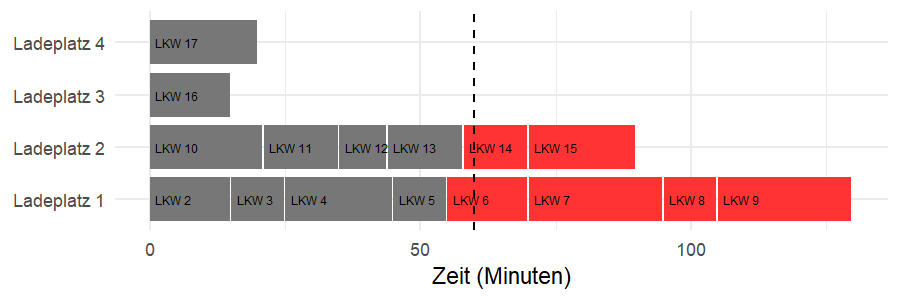
\includegraphics[width=\textwidth]{images/timelines/timelineTspCutExample1.png}
    \caption{Beispiel für einen per mTSP sortierten Zeitplan}
    \label{fig:tspCutExample1}
\end{figure}

In Abbildung \ref{fig:tspCutExample2} ist der Zeitplan aus Abbildung \ref{fig:tspCutExample1} auf einen 60 Minuten Slot angepasst worden. Zuerst wurden LKW 14 und LKW 15 vom Ladeplatz 2 entfernt und auf Ladeplatz 4 verschoben, da dies die einzige Kette ist, die noch vollständig auf einen anderen Platz passt. Die Kette von LKW 6 bis LKW 9 wurde auf Ladeplatz 3 verschoben, hier ist allerdings zu erkennen, dass diese dort nicht komplett hinein passt und somit LKW 8 und LKW 9 in dem gesamten Slot nicht mehr bearbeitet werden können. Außerdem haben sich die Zeitfenster der LKW am Anfang und Ende der zusammenhängenden Ketten leicht verlängert, da sowohl die verschobenen Teile, als auch die zurückgebliebenen Teile etwas längere Zeit brauchen, da hier kein optimaler Wechsel der Ladehilfsmittel mehr gegeben ist.

\begin{figure}[H]
    \centering
    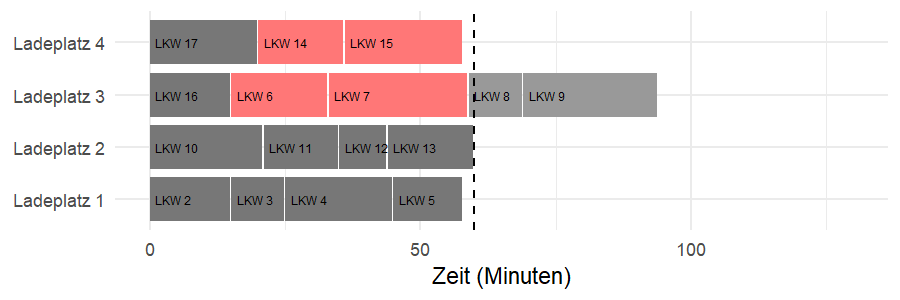
\includegraphics[width=\textwidth]{images/timelines/timelineTspCutExample2.png}
    \caption{Zeitplan aus Abb. \ref{fig:tspCutExample1} auf einen 60 Minuten Slot angepsst}
    \label{fig:tspCutExample2}
\end{figure}


\subsubsection{Vergleichswerte zur Auswertung generieren}
\label{sec:konzeptTspVergleichswerte}

\todo{fcfs ausgangssituation generieren beschreiben}

Ein letzter Schritt, welcher nicht direkt für den zuvor beschriebenen Optimierungsalgorithmus benötigt wird, ist die Generierung eines Zeitplans zu Vergleichs- und Auswertungszwecken. Dieser Zeitplan soll die Reihenfolge der Abfertigung im unoptimierten Zustand nachbilden. Nötig ist dies, da kaum nutzbare, reale Testdaten vorhanden sind. Gerade um eine große Menge generierter LKW Buchungen auswerten zu können, macht es durchaus Sinn sich Gedanken zu machen, wie ein solcher Algorithmus arbeiteten könnte. Zusätzlich lassen sich hier auch noch einmal genaue Erkenntnisse und ein besseres Verständnis für die bisherige Ausgangssiuation gewinnen, wenn man sich klar macht, wie die LKW dort ankommen.

Prinzipiell kommen die LKW nach keinem wirklichen System an, wie bereits in Kapitel \ref{sec:analyse} herausgearbeitet wurde. Innerhalb des Slots kommen die LKWs theoretisch zu einer zufälligen Zeit. Somit wäre der Ansatz hier, die Liste der ankommenden LKW in eine zufällige Reihenfolge zu bringen und diese nach dem \glqq{}first come, first served\grqq{}-Prinzip zu sortieren. Für einen Ladeplatz ist da nicht viel Logik nötig, die Liste kann genau in dieser Reihenfolge übernommen werden. Für mehrere Ladeplätze müsste hier auch wieder die Zeitberechnung aus dem Optimierungsalgorithmus (siehe Kapitel \ref{sec:berechnungGraphenTsp}) herangezogen werden. Für die vorliegende Lösung wurde angenommen, dass die Abfertigungszeit, die jede Maschine braucht, sich nicht verändert. Ein Vorteil wird durch die beste Reihenfolge und die Einsparung von Fahrt- und Rüstzeiten erreicht. Das System zur Kostenberechnung selbst kann somit auch hier eingesetzt werden. Es müsste bei der Sortierung auf mehrere Plätze also nach jedem einsortierten LKW die entsprechende Dauer bis zur Fertigstellung des bisher letzten LKW berechnet werden und anschließend immer zum Ladeplatz mit der kürzesten Dauer ein LKW einsortiert werden. So wird nachgebildet, dass immer der Ladeplatz welcher als nächstes frei wird, den nächsten LKW aufnimmt.

Insgesamt lässt sich so eben auch genau das Ausgangsproblem nachbilden: Die LKW kommen wie sie wollen, es wird keine Rücksicht darauf genommen, welche Ressourcen benötigt werden. Somit kann es zufällig einmal passen, dass die richtige Maschine bereits Vorort ist, in der Regel wird dies aber nicht der Fall sein und somit ein hoher Wechselaufwand entstehen.
